\documentclass[12pt,a4paper]{book}
\usepackage{lmodern}
\usepackage[svgnames]{xcolor} % Required to specify font color
\input{styles/couleurs.tex}
\usepackage[utf8]{inputenc} 
\usepackage[T1]{fontenc}
\usepackage{wrapfig}
\usepackage[french, english]{babel}
\usepackage[top=1.7cm, bottom=1.7cm, left=1.7cm, right=1.7cm]{geometry}
\usepackage{verbatim}
\usepackage{tikz} %Vectoriel
\usepackage{listings}
\usepackage{fancyhdr}
\usepackage{multido}
\usepackage{amssymb}
\usepackage{float}
\usepackage{titlebox}
\usepackage[francais]{minitoc}
\usepackage[final]{pdfpages} 
\usepackage{graphicx} % Required for box manipulation
\usepackage{epstopdf}
\usepackage{titletoc}
%\usepackage{makeidx}
\usepackage{imakeidx}
%\usepackage[totoc]{idxlayout}
\indexsetup{level=\chapter,toclevel=chapter}
\usepackage[urlbordercolor={1 1 1}, linkbordercolor={1 1 1}, linkcolor=black, urlcolor=bleu, colorlinks=true]{hyperref}

\makeindex


\newcommand{\titre}{Développement d'un outil de tests pour un logiciel de contrôle moteur}
\newcommand{\subtitle}{GreenT}
\newcommand{\auteur}{Antoine de \bsc{Roquemaurel}}
\newcommand{\semestre}{6}
\newcommand{\annee}{2014}
\newcommand{\putminitoc}{%
\begin{wrapfigure}{r}{0.60\textwidth}
\vspace{-15px}
\begin{tocBox}
\hspace{-30px}
\begin{minipage}{1.1\textwidth}
\minitoc~
\end{minipage}
\end{tocBox}
\end{wrapfigure}
}

\usepackage{geometry}
\usepackage{amsmath}
\usepackage[some]{background}
\usepackage{lipsum}

\newcommand{\pole}{}

\definecolor{gris1}{gray}{0.40}
\definecolor{gris2}{gray}{0.55}
\definecolor{gris3}{gray}{0.65}
\definecolor{gris4}{gray}{0.50}
\definecolor{vert}{rgb}{0,0.4,0}
\definecolor{violet}{rgb}{0.65, 0.2, 0.65}
\definecolor{bleu1}{rgb}{0,0,0.8}
\definecolor{bleu2}{rgb}{0,0.2,0.6}
\definecolor{bleu3}{rgb}{0,0.2,0.2}
\definecolor{rouge}{HTML}{F93928}


\lstdefinelanguage{algo}{%
   morekeywords={%
    %%% couleur 1
		importer, programme, glossaire, fonction, procedure, constante, type, 
	%%% IMPORT & Co.
		if, then, endif, else, si, sinon, alors, fin, tantque, debut, faire, lorsque, fin lorsque, 
		declenche, declencher, enregistrement, tableau, retourne, retourner, =, pour, a,
		/=, <, >, traite,exception, 
	%%% types 
		Entier, Reel, Booleen, Caractere, Réél, Booléen, Caractère,
	%%% types 
		entree, maj, sortie,entrée,
	%%% types 
		et, ou, non,
	},
  sensitive=true,
  morecomment=[l]{--},
  morestring=[b]',
}

\lstset{language=algo,
    %%% BOUCLE, TEST & Co.
      emph={importer, programme, glossaire, fonction, procedure, constante, type},
      emphstyle=\color{bleu2},
    %%% IMPORT & Co.  
	emph={[2]
		if, then, endif, else, eval, pre, si, sinon, alors, fin , tantque, debut, faire, lorsque, fin lorsque, 
		declencher, retourner, et, ou, non,enregistrement, retourner, retourne, 
		tableau, /=, <, =, >, traite,exception, pour, a
	},
      emphstyle=[2]\color{bleu1},
    %%% FONCTIONS NUMERIQUES
     % emph={[3]Entier, Reel, Booleen, Caractere, Booléen, Réél, Caractère},
      emphstyle=[3]\color{gris1},
    %%% FONCTIONS NUMERIQUES
      emph={[4]entree, maj, sortie, entrée},	
      emphstyle=[4]\color{gris1},
}
\lstdefinelanguage{wl}{%
   morekeywords={%
    %%% couleur 1
		importer, programme, glossaire, fonction, procedure, constante, type, 
	%%% IMPORT & Co.
		si, sinon, alors, fin, TANTQUE, tantque, FIN, PROCEDURE, debut, faire, lorsque, 
		fin lorsque, declenche, declencher, enregistrement, tableau, retourne, retourner, =, 
		/=, <, >, traite,exception, 
	%%% types 
		Entier, Reel, Booleen, Caractere, Réél, Booléen, Caractère,
	%%% types 
		entree, maj, sortie,entrée,
	%%% types 
		et, ou, non,
	},
  sensitive=true,
  morecomment=[l]{//},
  morestring=[b]',
}

\lstset{language=wl,
    %%% BOUCLE, TEST & Co.
      emph={importer, programme, glossaire, fonction, procedure, constante, type},
      emphstyle=\color{bleu2},
    %%% IMPORT & Co.  
	emph={[2]
		si, sinon, alors, fin , tantque, debut, faire, lorsque, fin lorsque, 
		declencher, retourner, et, ou, non,enregistrement, retourner, retourne, 
		tableau, /=, <, =, >, traite,exception
	},
      emphstyle=[2]\color{bleu1},
    %%% FONCTIONS NUMERIQUES
%      emph={[3]Entier, Reel, Booleen, Caractere, Booléen, Réél, Caractère},
 %     emphstyle=[3]\color{gris1},
    %%% FONCTIONS NUMERIQUES
      emph={[4]entree, maj, sortie, entrée},	
      emphstyle=[4]\color{gris1},
}
\lstdefinelanguage{css}{%
   morekeywords={%
    %%% couleur 1
		background, image, repeat, position, index, color, border, font, 
		size, url, family, style, variant, weight, letter, spacing, line, 
		height, text, decoration, align, indent, transform, shadow, 
		background, image, repeat, position, index, color, border, font, 
		size, url, family, style, variant, weight, letter, spacing, line, 
		height, text, decoration, align, indent, transform, shadow, 
		vertical, align, white, space, word, spacing,attachment, width, 
		max, min, margin, padding, clip, direction, display, overflow,
		visibility, clear, float, top, right, bottom, left, list, type, 
		collapse, side, empty, cells, table, layout, cursor, marks, page, break,
		before, after, inside, orphans, windows, azimuth, after, before, cue, 
		elevation, pause, play, during, pitch, range, richness, spek, header, 
		numeral, punctuation, rate, stress, voice, volume,
	%%% types 
		left, right, bottom, top, none, center, solid, black, blue, red, green,
	},
  sensitive=true,
  sensitive=true,
  morecomment=[s]{/*}{*/},
  morestring=[b]',
}
\lstset{language=css,
    %%% BOUCLE, TEST & Co.
      emph={
		background, image, repeat, position, index, color, border, font, 
		size, url, family, style, variant, weight, letter, spacing, line, 
		height, text, decoration, align, indent, transform, shadow, 
		background, image, repeat, position, index, color, border, font, 
		size, url, family, style, variant, weight, letter, spacing, line, 
		height, text, decoration, align, indent, transform, shadow, 
		vertical, align, white, space, word, spacing,attachment, width, 
		max, min, margin, padding, clip, direction, display, overflow,
		visibility, clear, float, top, right, bottom, left, list, type, 
		collapse, side, empty, cells, table, layout, cursor, marks, page, break,
		before, after, inside, orphans, windows, azimuth, after, before, cue, 
		elevation, pause, play, during, pitch, range, richness, spek, header, 
		numeral, punctuation, rate, stress, voice, volume,
	  },
      emphstyle=\color{bleu2},
    %%% FONCTIONS NUMERIQUES
      emph={[3]
		left, right, bottom, top,none, solid, black, blue, green,
		  },
      emphstyle=[3]\color{bleu3},
    %%% FONCTIONS NUMERIQUES
}

\lstset{language=SQL,
    %%% BOUCLE, TEST & Co.
      emph={INSERT, UPDATE, DELETE, WHERE, SET, GROUP, BY, ORDER, REFERENCES},
      emphstyle=\color{bleu2},
    %%% IMPORT & Co.  
	emph={[2]
		if, end, begin, then, for, each, else, after, of, on, to
	},
      emphstyle=[2]\color{bleu1},
    %%% FONCTIONS NUMERIQUES
%      emph={[3]Entier, Reel, Booleen, Caractere, Booléen, Réél, Caractère},
 %     emphstyle=[3]\color{gris1},
    %%% FONCTIONS NUMERIQUES
      emph={[4]entree, maj, sortie, entrée},	
      emphstyle=[4]\color{gris1},
}
\lstdefinelanguage{ARM}{%
   morekeywords={%
   ADD, SUB, MOV, MUL, RSB,CMP, BLS, BLE, B,BHI,LDR,
   BGE, RSBLT, BGT, BEQ, BNE,BLT,BHS,STR,STRB,ADR, LDMFD, STMFD, LDRB
	},
  sensitive=true,
  morecomment=[l]{@},
  morestring=[b]',
}

\lstdefinelanguage{javascript}{
   morekeywords={%
		if, while, else
	},
  sensitive=true,
  comment=[s]{/*}{*/},
  morecomment=[l]{//},
  string=[b]',
  morestring=[b]",
}
\lstdefinelanguage{PHP}{
   morekeywords={%
	foreach, echo, include, div, a, as, return, while, function, array
	},
  sensitive=true,
  morecomment=[s]{<!--}{-->},
  morecomment=[s]{/*}{*/},
  morecomment=[l]{//},
  string=[b]',
  morestring=[b]",
}
\lstset{language=Caml,
    %%% BOUCLE, TEST & Co.
      emph={int,bool, float},
      emphstyle=\color{bleu2},
}

\lstset{ % general style for listings 
   numbers=left 
   , literate={é}{{\'e}}1 {è}{{\`e}}1 {à}{{\`a}}1 {ê}{{\^e}}1 {É}{{\'E}}1 {ô}{{\^o}}1 {€}{{\euro}}1{°}{{$^{\circ}$}}1 {ç}{ {c}}1 {ù}{u}1
	, extendedchars=\true
   , tabsize=2 
   , stepnumber=2
   , frame=l
   , framerule=1.1pt
   , linewidth=510px
   , breaklines=true 
   , basicstyle=\footnotesize\ttfamily 
   , numberstyle=\tiny\ttfamily 
   , framexleftmargin=0mm 
   , xleftmargin=0mm 
   , captionpos=b 
	, keywordstyle=\color{bleu2}
	, commentstyle=\color{vert}
	, stringstyle=\color{rouge}
	, showstringspaces=false
	, extendedchars=true
	, mathescape=false
	, prebreak=\raisebox{0ex}[0ex][0ex]
		   {\ensuremath{\hookleftarrow}}
	,breakatwhitespace=true
} 
%	\lstlistoflistings
%	\addcontentsline{toc}{part}{List of code examples}

%	THEOREM STYLES
%----------------------------------------------------------------------------------------

\usepackage{amsmath,amsfonts,amssymb,amsthm} % For including math equations, theorems, symbols, etc

\newcommand{\intoo}[2]{\mathopen{]}#1\,;#2\mathclose{[}}
\newcommand{\ud}{\mathop{\mathrm{{}d}}\mathopen{}}
\newcommand{\intff}[2]{\mathopen{[}#1\,;#2\mathclose{]}}
\newtheorem{notation}{Notation}[chapter]

\newtheoremstyle{ocrenum} % Theorem style name
{7pt} % Space above
{7pt} % Space below
{\normalfont} % Body font
{} % Indent amount
{\small\bf\sffamily\color{ocre}} % Theorem head font
{\;\;} % Punctuation after theorem head
{0.25em} % Space after theorem head
{\small\sffamily\color{ocre}\thmname{#1}\thmnumber{} % Theorem text (e.g. Theorem 2.1)
\thmnote{\ {\the\thm@notefont\sffamily\bfseries\color{black}--- #3.}}} % Optional theorem note
\renewcommand{\qedsymbol}{$\blacksquare$} % Optional qed square

\newtheoremstyle{blacknumex} % Theorem style name
{7pt} % Space above
{7pt} % Space below
{\normalfont} % Body font
{} % Indent amount
{\small\bf\sffamily} % Theorem head font
{\;\;} % Punctuation after theorem head
{0.25em} % Space after theorem head
{\small\sffamily{\tiny\ensuremath{\blacksquare}}\ \thmname{#1}\thmnumber{\@ifnotempty{#1}{ }\@upn{#2}} % Theorem text (e.g. Theorem 2.1)
\thmnote{\ {\the\thm@notefont\sffamily\bfseries--- #3.}}} % Optional theorem note

\newtheoremstyle{blacknum} % Theorem style name
{7pt} % Space above
{7pt} % Space below
{\normalfont} % Body font
{} % Indent amount
{\small\bf\sffamily} % Theorem head font
{\;\;} % Punctuation after theorem head
{0.25em} % Space after theorem head
{} % Optional theorem note
\makeatother

% Defines the theorem text style for each type of theorem to one of the three styles above
\theoremstyle{ocrenum}
\newtheorem{theoremeT}{Theorem}[chapter]
\newtheorem{proposition}{Proposition}[chapter]
\newtheorem{problem}{Problem}[chapter]
\newtheorem{attentionT}{}[chapter]
\theoremstyle{blacknum}
\newtheorem{exampleT}{Example}[chapter]
\newtheorem{vocabulary}{Vocabulary}[chapter]
\newtheorem{definitionT}{Definition}[chapter]
\newtheorem{remarqueT}{}[chapter]
\newtheorem{exempleT}{}[chapter]




%----------------------------------------------------------------------------------------
%	DEFINITION OF COLORED BOXES
%----------------------------------------------------------------------------------------

\RequirePackage[framemethod=default]{mdframed} % Required for creating the theorem, definition, exercise and corollary boxes

% Theorem box
\newmdenv[skipabove=7pt,
skipbelow=7pt,
backgroundcolor=black!5,
linecolor=ocre,
innerleftmargin=5pt,
innerrightmargin=5pt,
innertopmargin=5pt,
leftmargin=0cm,
rightmargin=0cm,
innerbottommargin=5pt]{tBox}

\newmdenv[skipabove=0pt,
skipbelow=0pt,
backgroundcolor=black!2,
linecolor=black,
innerleftmargin=0pt,
innerrightmargin=0pt,
innertopmargin=0pt,
leftmargin=0cm,
rightmargin=0cm,
innerbottommargin=0pt]{tocBox}

% Exercise box	  
\newmdenv[skipabove=7pt,
skipbelow=7pt,
rightline=false,
leftline=true,
topline=false,
bottomline=false,
backgroundcolor=ocre!10,
linecolor=ocre,
innerleftmargin=5pt,
innerrightmargin=5pt,
innertopmargin=5pt,
innerbottommargin=5pt,
leftmargin=0cm,
rightmargin=0cm,
linewidth=4pt]{eBox}	

% Definition box
\newmdenv[skipabove=10pt,
skipbelow=10pt,
rightline=false,
leftline=true,
topline=false,
bottomline=false,
linecolor=ocre,
innerleftmargin=5pt,
innerrightmargin=5pt,
innertopmargin=0pt,
leftmargin=0cm,
rightmargin=0cm,
linewidth=4pt,
innerbottommargin=0pt]{dBox}	

% Corollary box
\newmdenv[skipabove=7pt,
skipbelow=7pt,
rightline=false,
leftline=true,
topline=false,
bottomline=false,
linecolor=gray,
backgroundcolor=black!5,
innerleftmargin=5pt,
innerrightmargin=5pt,
innertopmargin=5pt,
leftmargin=0cm,
rightmargin=0cm,
linewidth=4pt,
innerbottommargin=5pt]{cBox}		

% Corollary box
\newmdenv[skipabove=7pt,
skipbelow=7pt,
rightline=true,
leftline=false,
topline=false,
bottomline=true,
linecolor=gray,
backgroundcolor=black!5,
innerleftmargin=5pt,
innerrightmargin=5pt,
innertopmargin=5pt,
leftmargin=0cm,
rightmargin=0cm,
linewidth=1pt,
innerbottommargin=5pt]{rBox}				  
		  
% Corollary box
\newmdenv[skipabove=7pt,
skipbelow=7pt,
rightline=false,
leftline=true,
topline=false,
bottomline=false,
backgroundcolor=vertfonce!7,
linecolor=vertfonce,
innerleftmargin=5pt,
innerrightmargin=5pt,
innertopmargin=5pt,
innerbottommargin=5pt,
leftmargin=0cm,
rightmargin=0cm,
linewidth=4pt]{gBox}			  

% Creates an environment for each type of theorem and assigns it a theorem text style from the "Theorem Styles" section above and a colored box from above
\newenvironment{theorem}{\begin{tBox}\begin{theoremeT}}{\end{theoremeT}\end{tBox}}
\newenvironment{example}{\begin{exampleT}}{\hfill{\tiny\ensuremath{\blacksquare}}\end{exampleT}}
\newenvironment{definition}{\begin{dBox}\begin{definitionT}}{\end{definitionT}\end{dBox}}
\newenvironment{attention}{\begin{eBox}\small}{\end{eBox}}				  	
\newenvironment{remarque}{\begin{cBox}\textbf{\color{gray}Remarque}\small}{\end{cBox}}	
\newenvironment{exemple}{\begin{gBox}\textbf{\color{vert}Exemple}\small}{\end{gBox}}	

%----------------------------------------------------------------------------------------
%	REMARK ENVIRONMENT
%----------------------------------------------------------------------------------------

%\newenvironment{remarque}{\par\vskip10pt\small
%\begin{rBox}
%\begin{list}{}{
%\leftmargin=35pt % Indentation on the left
%\rightmargin=25pt}\item\ignorespaces % Indentation on the right
%%\makebox[-2.5pt]{\begin{tikzpicture}[overlay]
%%\node[draw=ocre!60,line width=1pt,circle,fill=ocre!25,font=\sffamily\bfseries,inner sep=2pt,outer sep=0pt] at %(-15pt,0pt){\textcolor{ocre}{R}};\end{tikzpicture}} % Orange R in a circle
%\advance\baselineskip -1pt}
%{\end{list}\vskip1mm\end{rBox}\vskip5pt} % Tighter line spacing and white space after remark



\DeclareTextFontCommand{\policeGlossaire}{\fontfamily{lmss}\selectfont}
\DeclareTextFontCommand{\policePackage}{\fontfamily{phv}\selectfont}
\DeclareTextFontCommand{\policeTitre}{\fontfamily{ptm}\selectfont}
\newcommand{\policeCode}[1]{\texttt{#1}}

\newcommand{\sectionfont}{%
	\fontencoding{\encodingdefault}%
	\fontfamily{pag}%
	\fontseries{bc}%
	\fontshape{n}%
	\selectfont
}

% numéro du chapitre
\DeclareFixedFont{\chapnumfont}{T1}{phv}{b}{n}{80pt}
% pour le mot « Chapitre »
\DeclareFixedFont{\chapchapfont}{T1}{phv}{b}{n}{16pt}
% pour le titre
\DeclareFixedFont{\chaptitfont}{T1}{phv}{b}{n}{24.88pt}


\usepackage[explicit]{titlesec}
\usepackage{lmodern}

\newlength\chapnumb
\setlength\chapnumb{4cm}

\titleformat{\chapter}[block]
{\normalfont\sffamily}{}{0pt}
{\parbox[b]{\chapnumb}{%
\vspace{-80px}%
   \fontsize{85}{110}\selectfont\thechapter}%
  \parbox[b]{\dimexpr\textwidth-\chapnumb\relax}{%
    \raggedleft%
    \hfill{\Huge#1}\\
    \rule{\dimexpr\textwidth-\chapnumb\relax}{0.4pt}}}
\titleformat{name=\chapter,numberless}[block]
{\normalfont\sffamily}{}{0pt}
{\parbox[b]{\chapnumb}{%
   \mbox{}}%
  \parbox[b]{\dimexpr\textwidth-\chapnumb\relax}{%
    \raggedleft%
    \hfill{\Huge#1}\\
    \rule{\dimexpr\textwidth-\chapnumb\relax}{0.4pt}}}


\makeatletter

\newlength{\sectiontitleindent}
\newlength{\subsectiontitleindent}
\newlength{\subsubsectiontitleindent}
\setlength{\sectiontitleindent}{-1cm}
\setlength{\subsectiontitleindent}{-.5cm}
\setlength{\subsubsectiontitleindent}{-.25cm}

\renewcommand{\section}{%
  \@ifstar{%
\@startsection%
{section}%
{1}%
{\sectiontitleindent}%
{-3.5ex plus -1ex minus -.2ex}%
{2.3ex plus.2ex}%
{\sectionfont\Large}
	    }{%
\@startsection%
{section}%
{1}%
{\sectiontitleindent}%
{-3.5ex plus -1ex minus -.2ex}%
{2.3ex plus.2ex}%
{\sectionfont\Large}
  }%
}
\renewcommand{\subsection}{%
	\@startsection%
	{subsection}%
	{2}%
	{\subsectiontitleindent}%
	{-3.5ex plus -1ex minus -.2ex}%
	{2.3ex plus.2ex}%
	{\sectionfont\large}
}

\renewcommand{\subsubsection}{%
	\@startsection%
	{subsubsection}%
	{3}%
	{\subsubsectiontitleindent}%
	{-1.5ex plus -1ex minus -.2ex}%
	{0.5ex plus.2ex}%
	{\sectionfont\normalsize}
}

\makeatother

\newcommand{\lien}[1]{
 $\vartriangleright$ \url{#1}
 }

\input{styles/headers.tex}

\mtcsettitle{minitoc}{\hfill Sommaire}
\mtcsetrules{minitoc}{off}
\mtcsetfeature{minitoc}{before}{\vspace{0pt}}% à ajuster
\mtcsetfeature{minitoc}{after}{\vspace{-25pt}}% à ajuster

\makeatother
\includeonly {
	contents/intro,
	contents/abstract,
	contents/conti/conti,
	contents/organization/organization,
	contents/problem/problem,
%
	contents/greent/greent,
	contents/greent/collaboration,
	contents/bilan/bilan,
%
	annexes/glossary,
	annexes/references,	
%	annexes/devices,	
	annexes/generatesFiles,
	annexes/report,
	annexes/releasenote
}


\begin{document}
	\setcounter{tocdepth}{1}
	\setcounter{secnumdepth}{2}
	\setcounter{minitocdepth}{1}
	
	\begin{titlepage}
\BgThispage
\SetBgScale{1}
\SetBgAngle{0}
\SetBgOpacity{1}
\SetBgContents{\begin{tikzpicture}[remember picture,overlay]
	 \path [fill=titlepagecolor] (-0.5\paperwidth,1.5) rectangle (0.5\paperwidth,9);  
 \end{tikzpicture}}
\newgeometry{top=3cm,left=1cm,right=1cm,bottom=2cm}
\begin{tabular}{cp{1.8cm}c}
	\begin{minipage}{0.4\textwidth}
		\vspace{-60px}
		\hspace{-35px}
		\includegraphics[width=8cm]{styles/images/logos/ups.jpg}
		\includegraphics[width=8cm]{styles/images/logos/mdl.png}
	\end{minipage}
	&
	&
	\begin{minipage}{0.4\textwidth}
		\vspace{-40px}
		\includegraphics[height=3cm]{styles/images/logos/conti.png}
	\end{minipage}
	\\
\end{tabular}

\vspace*{0.1\textheight}
\noindent
\textcolor{white}{
\fontfamily{phv}\selectfont
%\vspace{-20px}
	\fontsize{38}{38}\textbf{\textsf{Rapport de stage}}
%	\vspace{25px}
%	\newline
\fontfamily{ptm}\selectfont
\begin{center}
	\Huge Développement d'un outil de tests pour un logiciel de contrôle moteur:\newline
\end{center}
	\vspace{-60px}
	\begin{center}
		\Huge
	GreenT
	\end{center}
}
\vspace*{2cm}\par
\noindent
\vfill
\begin{center}
	\par\normalfont\sffamily\selectfont
	\vspace{-100px}
	\Huge
	Antoine de \bsc{Roquemaurel}\\
	\vspace{30px}
	\Large
	M2 Informatique -- Développement Logiciel\\
	2015 -- 2016
\end{center}
\vfill
\begin{tabular}{lp{3.6cm}r}
	\begin{minipage}{0.3\textwidth}
		\large
	Maître de stage:\newline Alain \bsc{Fernandez}\newline\newline
	Tuteur universitaire:\newline Jean-Baptiste \bsc{Raclet}
	\end{minipage}
	& &
	\begin{minipage}{0.46\textwidth}
		\begin{flushright}
			\large
		Du 14 Septembre 2015 au 30 Août 2016\newline
		\footnotesize
		Version du \today~
	\end{flushright}
	\end{minipage}
	\\

\end{tabular}
\end{titlepage}

	~\newpage
	\addcontentsline{toc}{chapter}{Remerciements} 
	~
	\vfill
	\begin{flushright}
		\begin{minipage}{0.7\textwidth}
			Je tiens à remercier toutes les personnes m'ayant permis de réaliser ce stage.\\~

En premier lieu, un grand merci à Corinne \bsc{Tarin} pour m'avoir accepté au sein de son équipe.

Je remercie particulièrement Alain \bsc{Fernandez} pour m'avoir suivi et conseillé tout au long de ce stage.

Une pensée à Joelle \bsc{Decol} pour sa bonne humeur quotidienne, ainsi qu'à toute l'équipe du troisième étage, grâce à qui j'ai passé d'excellents moments au sein de l'entreprise.

Merci à mon tuteur universitaire Joseph \bsc{Boudou} pour son suivi et sa visite en entreprise.

Enfin, je remercie toutes les personnes m'ayant entouré durant ce stage et aidé à la rédaction ce rapport, à savoir Diane, Ophélie, Clément et Mathieu.

		\end{minipage}
	\end{flushright}
	\vfill
	~
	\chapter*{Résumé}
\addcontentsline{toc}{chapter}{Résumé} 
\vspace{-45px}
\footnotesize{\textbf{Mots-clés}: Automobile, Outil, ECU, Contrôle moteur, Tests, Banc de tests, HiL, Debugger, Java, Python}

\normalsize
Dans le cadre de ma formation en seconde année de Master Développement Logiciel à l'université
Toulouse III, j'ai eu la chance de pouvoir effectuer un an d'alternance. J'ai eu l'opportunité de continuer un projet commencé précédemment : le développement
d'un outil de tests de logiciels embarqués.

L'entreprise Continental est une Société Allemande leader de l'automobile possédant plus de $170\;000$
employés dans le monde. L'entreprise s'occupe aussi bien des calculateurs que de la sécurité automobile,
du système d'injection, \ldots\newline
Pour ma part j'ai travaillé au sein de l'équipe en charge de la mise en place de services de tests.
Notamment des tests logiciels, ceci en développant des scripts de tests automatique de non-régression
ou d'intégration avant la livraison des projets.

Trois ans avant ce stage, un besoin a été exprimé : pouvoir tester de façon rapide et efficace
l'intégration d'un « plugin », un bout de code sous forme binaire, au sein des applicatifs d'un calculateur de contrôle moteur. La mission de l'équipe \textit{Tests \& Automation Service} est de permettre
de tester la bonne intégration de ce plugin avec les logiciels Continental. Pour cela le développement
d'un outil de tests est nécessaire.

Au début de mon alternance, cet outil appelée GreenT, avait déjà était bien avancée, en partie lors de mes stage
précédent. Cependant, à mon arrivée un module devait être refondu afin de pouvoir livrer une première version de l'outil. Une fois celle-ci livrée, de nouvelles
fonctionnalités ainsi que du support de la maintenance étaient nécessaires. C'est donc dans ce contexte que j'ai
travaillé durant cette année, ceci afin d'améliorer au maximum l'outil, tout en accompagnant les utilisateurs.

Cet outil a pour but d'avoir des tests les plus exhaustifs et efficaces possibles. Afin de pouvoir
tester la bonne intégration du plugin, le client fourni un fichier Excel appelé Walkthrough contenant
la liste des variables du plugin avec toutes leur spécifications. Le testeur va ajouter des colonnes à ce
fichier afin de spécifier le fonctionnement du test, notre plateforme sera ensuite capable d'analyser
le fichier, et de générer les cas de tests qui s'exécuteront à distance sur un ou plusieurs bancs de
tests : ils simulent un environnement véhicule autour du contrôleur afin de vérifier ses réactions en
fonction des différentes conditions qui peuvent arriver.

%J'ai participé à l'ajout de deux nouvelles fonctionnalités : la possibilité de modifier des calibrations 1
%en début de stimulation, fonctionnalité indispensable à l'implémentation de certains tests. J'ai
%également développé un système permettant d'améliorer la généricité des tests, en autorisant l'utilisation
%de calibrations en tant qu'index de tableau, tel que tab[calibration].

Mon travail durant ce stage aura été bénéfique, pour l'entreprise grâce à mes connaissances de l'outil, 
au développement de nouvelles fonctionnalités, à mes corrections de bugs et au support que j'ai effectué. Mais aussi
personnellement, d'un point de vue technique, en trouvant des solutions à des problèmes. Et d'un
point de vue humain grâce au travail en équipe, aux comptes rendus réguliers qui m'ont permis
d'apprendre à synthétiser mon travail.

%Le projet n'est pas terminé, celui-ci est actuellement utilisé principalement pour des projets Ford, mais celui-ci doit être utilisé par les projets Renault prochainement. 
Le projet n'est pas terminé, celui-ci nécessitant encore de la maintenance et du développement de nouvelles fonctionnalités. Cependant, avec ces deux ans de travail, j'aurai eu l'opportunité de voir un cycle logiciel complet, allant de l'analyse des besoins jusqu'à l'exploitation de l'outil, ce qui sera un atout pour ma future carrière professionnelle.
%Le projet n'est pas terminé, et je vais continuer son développement dès Septembre en contrat de
%professionnalisation avec Continental, cette expérience supplémentaire va me permettre de connaître
%un cycle logiciel complet, ce qui sera un atout pour ma future carrière professionnelle.

%
%
{\let\cleardoublepage\relax\newpage
\chapter*{Abstract}}
\addcontentsline{toc}{chapter}{Abstract} 
\begin{otherlanguage}{english}
\textbf{Keywords}: Automotive, Tool, ECU, Control engine, Tests, Workbench, HiL, Debugger, Java, Python

During my second year of Master in computer science at Toulouse III University – Paul Sabatier,
I had the opportunity to do an internship. I chose to work in continuity of my 1st year, the development
of a tool for embedded tests, in Continental, an automotive company.

Continental is a leading German automotive manufacturing company who has 174 000 employees
all around the world. The company is specializing in tires, brake systems, automotive safety
and powertrain. I worked in the team that was in charge of software tests, with the development
and configuration of scripts. Those scripts are for regressions tests, and in my case, integration tests.

Three years before this internship, a need was been expressed: being able to quickly and efficiently
test the integration of a plugin, meaning a piece of code in binary. This plugin is for an
engine control software. The mission of the team Tests \& Automation Service is helping the proper
integration of this plugin with Continental software. For this purpose, the development of a test
tool is required.

The development of this tool, called GreenT, began three years ago. GreenT needs bugs corrections
and features development for production deployment. So, I worked in this context during
one year, and in january, the release 1.0 was deployed.

The goal of this tool was to provide the most exhaustive and effective tests possible. For
this purpose, the customer provides a specification file, called Walkthrough, wich contains the specification
of all plugin's variables. Testers will add columns in this file for test specification. After
this, GreenT will be able to parse and generate tests case that will be executed remotely on one
or several workbenches. A workbench can simulate a vehicle environment around an ECU to check
reactions.

I developed some features in this project: the improvement of reports generation, which is required for delivery, and systems 
for opening GreenT to most of projects. In addition, since january, I support users which writing tests.

So my work during this internship was beneficial for the company, my knowledge about GreenT
allowing me to help fixing bugs, and I was able to develop some new features, and help to delivery the first operational version of the tool.
It was also beneficial for me, from a technical point of view by designing solutions for particular
problems, and from a human point of view by improving my teamwork skills thanks to the meetings
we did to talk about the development.

This project is not completed yet, it required maintenance and development of new features. However, this two years of devlopment have shown me a complete software lifecycle, from needs analyze to exploitation of tool. It will be an asset for my future professional career.
\end{otherlanguage}
	\chapter*{Introduction}
	\addcontentsline{toc}{chapter}{Introduction} 


Dans le cadre de ma formation en première année de Master spécialité Développement Logiciel à l'université Toulouse III – Paul Sabatier, j'ai eu la possibilité d'effectuer un stage.


Attiré par le monde de l'entreprise et désireux de gagner en expérience, j'ai eu l'opportunité de continuer un projet commencé l'année précédente lors de mon stage de fin de Licence dans l'entreprise Continental Automotive : le développement d'une plateforme de tests de logiciels embarqués.

Ce projet a pour but d'aider une équipe de Continental, celle-ci est en charge de l'intégration d'un plugin, fourni sous forme binaire, que l'équipe doit intégrer dans le logiciel d'un calculateur de contrôle moteur. Pour cela, une plateforme permettant d'effectuer des tests automatisés est en développement.

Ayant connu les prémices de ce projet, et afin d'avoir un aperçu de celui-ci sur la longueur, allant de sa conception jusqu'à sa mise en production, le sujet du stage était particulièrement intéressant. En outre, celui-ci est en parfaite adéquation avec mon projet professionnel, et ma poursuite en M2 Développement Logiciel.

C'est au sein de l'équipe \textit{Test \& Automation Service} que j'ai effectué mon stage d'une durée de quatre mois, je vais ainsi vous présenter en quoi le développement de cet outil est nécessaire à l'équipe en charge des tests de ce plugin. Dans une première partie nous présenterons l'entreprise Continental et plus particulièrement l'équipe Tests \& Automation Service(chapitres \ref{chapConti} et \ref{chapOrganization}). Nous aborderons ensuite le problème que posent actuellement les tests de ce plugin(chapitre \ref{chapPb}), avant de présenter la solution qui est en cours de développement(chapitre \ref{chapGreent}) et comment j'ai contribué à ce projet(chapitre \ref{collab}). 

		\dominitoc

\tableofcontents

\setcounter{mtc}{4}
	\chapter{Continental}\label{chapConti}
\putminitoc
Mon stage s'est déroulé au sein de l'entreprise Continental. Cette entreprise est, sur les dernières années, entre première et deuxième équipementier automobile mondial par le volume de vente.

Ce chapitre présente rapidement le groupe Continental et plus particulièrement l'équipe \textit{Tests \& Automation Service} qui m'a accueilli pour ce stage.

	\section{Organisation de l'entreprise}
		\subsection{Le groupe Continental}

Continental est une entreprise allemande fondée en 1871 dont le siège se situe à Hanovre. Il s'agit d'une Société Anonyme (SA) dont le président du comité de
direction est le Dr. Elmar \bsc{Degenhart} depuis le 12 août 2009. Le groupe Continental est constitué de cinq divisions intervenant sur le marché des pneus (\textit{Rubben}) et de l'électronique automobile (\textit{Automotive}), ces divisions vous sont détaillés figure \ref{fig:repartitionConti}.
	 
		 \begin{figure}[H]
		 	\centering
		 	\includegraphics[width=17cm]{contents/images/caConti.png}
		 	\caption[Chiffre d'affaire et nombre d'employes (Annee 2014)]{Chiffre d'affaire et nombre d'employes (Annee 2014)\footnotemark{}}
		 	\label{fig:caConti}
		 \end{figure}
	 	\footnotetext{NAFTA : North American Free Trade Agreement}
		 En 2014, l'entreprise comptait plus de $189\;000$ employés dans le monde, comme le montre la figure\ref{fig:caConti} répartis dans 317 sites et 50 pays différents, dont la répartition est détaillée figure \ref{fig:repartitionConti}. Avec un chiffre d'affaire de 34.5 milliards d'euros au total, Continental est le numéro un du marché de production de pneus en Allemagne et est également un important équipementier automobile.

		 \begin{figure}[H]
		 	\centering
		 	\includegraphics[width=18cm]{contents/images/repartitionConti.png}
		 	\caption{Répartition du groupe Continental dans le monde}
		 	\label{fig:repartitionConti}
		 \end{figure}		 

		\subsection{Histoire de l'entreprise}
		Continental est fondée en 1871 comme société anonyme sous le nom de <<\textit{Continental-Caoutchouc-und Gutta-Percha Compagnie}>> par neuf banquiers et industriels de Hanovre (Allemagne).

		Continental dépose l'emblème du cheval représenté sur la figure \ref{fig:logo}, comme marque de fabrique à l'Office impérial des brevets de Hanovre en octobre 1882. Ce logo est aujourd'hui encore protégé en tant que marque distinctive.
		\begin{figure}[H]
			\centering
			\includegraphics[width=3cm]{contents/images/logoConti.png}
			\caption{Logo de Continental}
			\label{fig:logo}
		\end{figure}

		Le fabricant de pneus allemand débute son expansion à l'international en tant que sous-traitant automobile international en 1979, expansion qu'il n'a cessé de poursuivre depuis.
		
Entre 1979 et 1985, Continental procède à plusieurs rachats qui permettent son essor en Europe, celui des activités pneumatiques européennes de l'américain \textit{Uniroyal Inc.} et celui de l'autrichien \textit{Semperit}.

En 1995 est créée la division << \textit{Automotive Systems} >> pour intensifier les activités << systèmes >> de son industrie automobile.

La fin des années 1990 marque l'implantation de Continental en Amérique latine et en Europe de l'Est.

En 2001, pour renforcer sa position sur les marchés américain et asiatique, l'entreprise fait l'acquisition du spécialiste international de l'électronique \textit{Temic}, qui dispose de sites de production en Amérique et en Asie. La même année, la compagnie reprend la majorité des parts de deux entreprises japonaises productrices de composants d'actionnement des freins et de freins à disques. 

En 2004, le plus grand spécialiste mondial de la technologie du caoutchouc et des plastiques naît de la fusion entre \textit{Phoenix AG} et \textit{Conti'Tech}.

Enfin en juillet 2007, Continental réalise sa plus grosse opération en rachetant le fournisseur automobile \textit{Siemens VDO Automotive}. Ce rachat a permis à l'entreprise de multiplier son chiffre d'affaire par deux, passant ainsi de 13 milliards d'euros à plus de 34.5 milliards d'euros (chiffre de 2014).
		
		\subsection{Activités des différentes branches}
		\begin{figure}[H]
			\hspace{-55px}
			\includegraphics[width=21cm]{contents/images/structureConti.jpg}
			\caption{Structure de Continental}
			\label{fig:structConti}
		\end{figure}

		Comme on peut le voir sur la figure \ref{fig:structConti}, Continental est composée de cinq divisions. Ces dernières se chargent de développer et produire des équipements répondant aux besoins des clients. Pour cela elles sont composées de \textit{Business Units} qui ont chacune une activité bien particulière dans leur domaine de compétence. 

Durant mon stage, je travaillais au sein de \textit{P-ES} : 
\begin{description}
	\item[Division \textit{Powertrain}] S'occupe essentiellement du contrôle moteur, au niveau logiciel et matériel avec l'ECU\footnote{Engine Control Unit, Unité de calcul du contrôle moteur}
	\item[Business Unit \textit{Engine Systems}] Chargée de produire les équipements nécessaires au contrôle moteur tels que des calculateurs ou des injecteurs.
\end{description}

	\section{Le contexte de l'équipe TAS}
		J'ai travaillé dans l'équipe en charge des tests au niveau système ou logiciel dirigée par Corinne \bsc{Tarin}. Cette équipe doit aider à la vérification et la validation des programmes de contrôle moteur en fournissant des services de tests. 
		
 		\subsection{Le besoin} \label{besoinTests}
 		Le calculateur du contrôle moteur d'une voiture est un dispositif très important et à haut risque, en effet, une défaillance peut provoquer la mort de plusieurs personnes\footnote{Le programme d'une voiture comporte ainsi des fonctions dites << \textit{safety} >> tel que le régulateur, l'accélération, le freinage, \ldots}. Ainsi, le test est indispensable dans ce domaine, et doit être robuste. 

Le test des logiciel de contrôle moteur se fait aujourd'hui : 
\begin{itemize}
	\item << Soit à la main >> pour les tests d'intégration
	\item Soit à l'aide de scripts de test Python, écrit manuellement
\end{itemize}
Cependant, la taille des logiciels à tester est devenu particulièrement importante(Plusieurs milliers de variables, dans plus de 10 000 pages de spécifications\ldots). Cela appel à une automatisation plus forte des tests afin d'augmenter fortement la vitesse et la quantité de tests afin d'éliminer le maximum de bogue.

C'est dans ce contexte que l'équipe TAS intervient, c'est ainsi que je participe au développement d'un outil permettant d'automatiser des tests d'intégrations pour les équipes projet travaillant pour Ford.
 		\subsection{L'équipe Tests \& Automation Service}

 		% P : Powertrain
 		% ES : Engine System
 		% SE :
 		% CV :
 		% TAS : Test & Automation Service
 		% TODO ajouter schéma de l'équipe dans Powertrain ?
 		
 		Pour ma part, j'opérais dans la partie test automatique. Cette << sous-équipe >> possède deux missions : 
 		\begin{itemize}
 			\item Le développement et l'exécution de scripts de tests de non-régression\footnote{Aussi appelés FaST : \textbf{F}unctions \textbf{a}nd \textbf{S}oftware \textbf{T}esting}. Ces scripts de tests s'exécutent sur bancs HiL\footnote{\textbf{H}ardware \textbf{I}n the \textbf{L}oop. Vous trouverez plus d'explications sur ce dispositif section \ref{wb}} avant la livraison des projets
 			\item Le développement et la maintenance d'outils permettant d'améliorer la couverture et la qualité des tests. Ces outils doivent permettre aux développeurs de vérifier facilement et correctement leur travail, particulièrement pour des tests de non-régression bien que l'outil sur lequel je travail soit à destination de tests d'intégration.
 		\end{itemize}
	\subsection{Les outils de tests}
	Afin d'effectuer son travail, l'équipe TAS possède différents outils de tests. D'une part au niveau matériel avec des bancs de tests, mais aussi logiciel avec une plateforme écrite en Python.
	
		\subsubsection{Les bancs de tests}\label{wb}
		Afin de tester au mieux les programmes du contrôle moteur développés, ceux-ci sont d'abord testé via des simulateurs d'environnement véhicule. Ce simulateur permet de vérifier le programme avant d'effectuer des tests sur véhicule. Ces tests se font sur table dans un premier temps, pour deux raisons principales : 
		\begin{itemize}
			\item D'un part, les tables sont plus facilement accessible qu'un véhicule d'essais pour les équipes logicielles
			\item D'autre part, les tables possèdent plus de moyens afin d'observer finement l'ECU
		\end{itemize}
		
		Comme vous pouvez le voir figure \ref{fig:wb}, un banc de tests est composé d'un ordinateur, du calculateur appelé ECU pour \textit{\textbf{E}lectronic \textbf{C}ontrol \textbf{U}nit} et d'au moins deux équipements aidant aux tests. 
		
		Les deux équipements étant les suivants : 
		\begin{description}
			\item[Le HiL] Le \textit{\textbf{H}ardware \textbf{i}n the \textbf{L}oop} est un simulateur d'environnement véhicule. Ainsi l'ECU est branché sur le HiL et se comporte de la même manière que s'il était embarqué dans une voiture. Le HiL quant à lui est chargé d'envoyer les bons stimulus sur les pins de l'ECU, tel que l'injection, la vitesse de rotation du moteur, le starter \ldots
			\item[Debugger] Cet {appareil} est connecté au microcontrôleur de l'ECU via un port JTag. Il peut communiquer avec celui-ci afin d'effectuer différentes opérations. Tel que flasher le logiciel à tester, mettre des points d'arrêts sur le code, lire des variables, les modifier, changer des calibrations, \ldots
		\end{description}
	
		\begin{figure}[H]
			\centering
			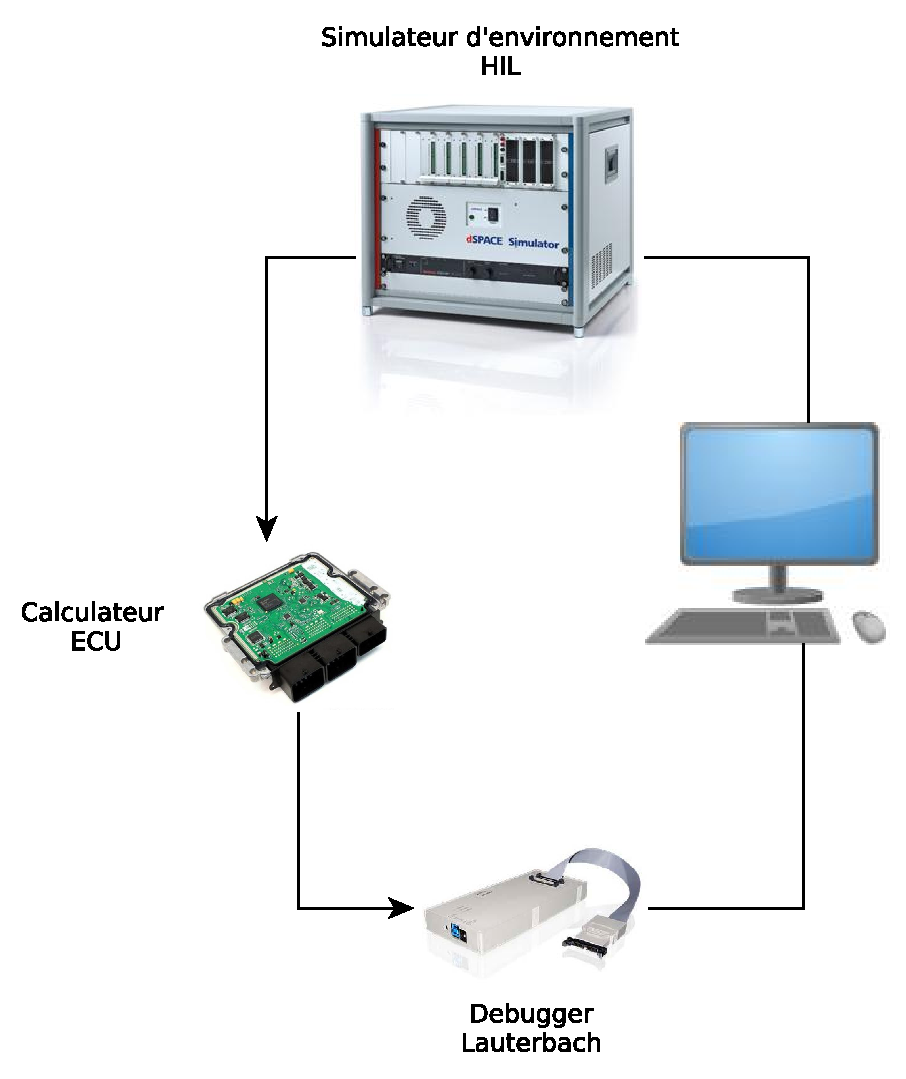
\includegraphics[width=12.1cm]{contents/images/WB.eps}
			\caption{Fonctionnement d'une table de tests : HIL DSpace, Debugger et ECU}
			\label{fig:wb}
		\end{figure}
				\begin{remarque}
					Un certain nombre d'équipes projet chez Continental utilise un troisième équipement qui n'est pas représenté ici, parce que notre plateforme ne s'en sert pas. Cet outil, nommé INCA, va interagir sur l'ECU via un bus CAN\footnote{Controller Area Network}.
				\end{remarque}
		Les différents équipements, ou \textit{device}, que nous pouvons voir sur cette figure sont ceux avec lesquelles notre nouvelle plateforme va communiquer afin d'effectuer des tests automatiques. 
		
			\subsubsection{La plateforme TA3}\label{ta3}
			\begin{wrapfigure}{l}{2.5cm}
				\includegraphics[width=2.5cm]{contents/images/python.png}
			\end{wrapfigure}
			Actuellement, les équipes de tests disposent d'une plateforme appelée TA3. Celle-ci est une bibliothèque de classes écrites en Python. Jusqu'à présent, pour chaque objectif de test, il fallait écrire un script python utilisant la TA3. Ces scripts pilotent le banc HIL et le debugger afin d'envoyer des stimulis à l'unité de contrôle moteur et de vérifier que les réactions de celui-ci sont conforme aux spécifications de test.
			
			Cependant, cette plateforme pose un certain nombre de problèmes qui rend son utilisation difficile. D'une part, elle renvoie un trop grand pourcentage de faux-positifs, faisant perdre du temps au testeur. D'autres part, elle ne prend pas en compte certains besoins apparu récemment comme par exemple un système permettant de flasher automatiquement les ECU\footnote{Cela permettrai de scripter un test qu'on lancerai plus tard et de gagner du temps}, ou la possibilité de vérifier la fréquence de mise-à-jour de la production de variables\footnote{Ceci afin de contrôler le temps réel du calculateur}.
			
			Afin d'améliorer cette situation, l'équipe \textit{Tests \& Automation Service} développe une nouvelle plateforme.
			
%C'est dans ce contexte que l'équipe \textit{Tests \& Automation Service} intervient, elle doit fournir des outils aux développeurs afin de vérifier facilement et correctement leur travail, particulièrement pour des tests de non-régression, bien que l'outil sur lequel je travaille soit à destination de tests d'intégration.
 % ok
\setcounter{mtc}{5}
	\chapter{Le problème} \label{chapPb}
\putminitoc
Depuis longtemps, l'entreprise avait un problème afin d'effectuer des tests d'intégrations, notamment pour les projets à destination de Ford. Les tests demandaient du temps et de l'argent à l'équipe en charge de ces tests. Ainsi, deux ans avant mon stage de M1, une solution à été trouvée : le développement d'une nouvelle plateforme, \textit{GreenT}.
	\section{\textit{Third-Party Software Component}}
	Étant donné la taille grandissante des programmes informatique, il est de plus en plus rare qu'une seule et unique entité effectue le développement d'un logiciel.
	
	C'est ainsi que chez Continental, un certain nombre de composant des calculateurs ne sont pas développés en interne. Ce concept est appelé \textit{Third-Party Software}. 
	
	La principale difficulté de ce mode de fonctionnement est l'intégration, une spécification exhaustive est indispensable afin de pouvoir connecter les différentes interfaces du composant avec le reste du projet. 
	
	C'est avec ces contraintes que travaillent l'équipe en charge du développement des différents logiciels de contrôle moteur à destination de Ford.
	
	\section{Les tests du << plugin >> Ford}\label{plugin}
	Dans le cadre de projets pour Ford, Continental ne développe pas l'intégralité du logiciel, une partie étant fournie par le client sous forme de << plugin >>. Ce plugin est un fichier binaire qui est chargé directement dans la mémoire flash de l'ECU sans que Continental n'ait accès au code source. Seule une description des interfaces est fournie. Le \textit{plugin} est supposé correct, et le tester n'est pas de notre ressort. Cependant, celui-ci va être interfacé avec les logiciels Continental : il est indispensable de vérifier que les deux parties fonctionnent ensemble lors de l'intégration.
	\begin{figure}[H]
		\centering
		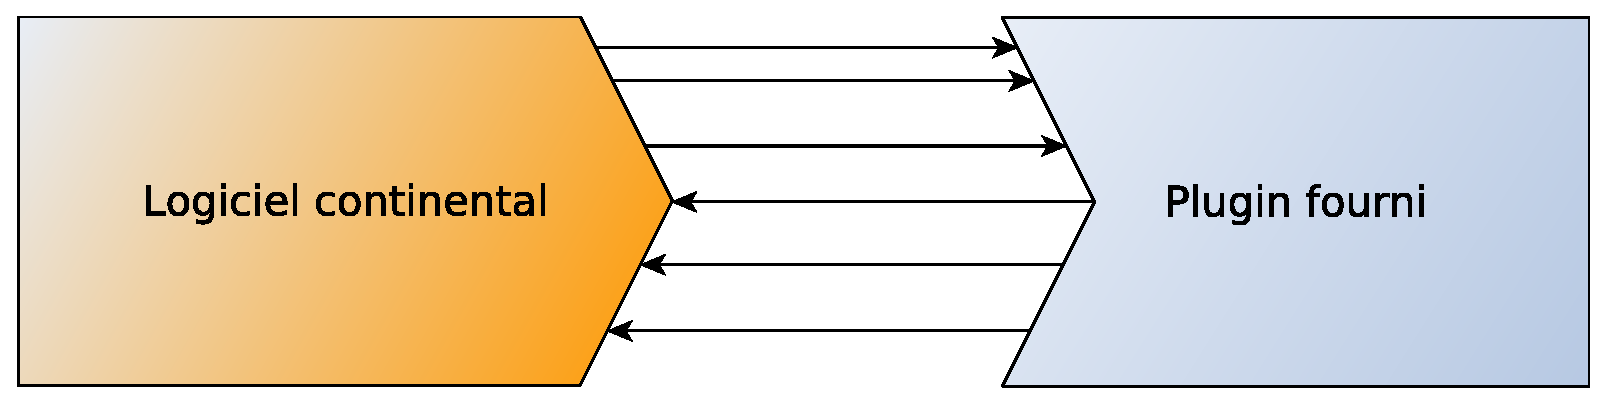
\includegraphics[width=8.0cm]{contents/images/plugin.eps}
		\caption{Interfaces du plugin avec le logiciel de Continental}
		\label{fig:plugin}	
	\end{figure}
	
	Le fichier de spécification est un fichier Excel, fourni par le client. Ce fichier, appelé \texttt{Walkthrough}\footnote{Ce fichier est expliqué plus en détail section \ref{wt}}, 
	contient la liste de toutes les variables du plugin avec toutes leur spécifications. Il contient
	environ 900 variables différentes. 
	
	Il est impensable de tester le fonctionnement d'autant de paramètres manuellement. Ainsi l'équipe en
	charge de tester cette intégration effectue des tests de différence d'une version à l'autre : seules les variables ayant pu être impactées par une \textit{release} seront testées, il est supposé que le fonctionnement des autres variables reste inchangé. Ce type de test est appelé \textit{Delta Test}.
	
	\vspace{20px}
	Deux problèmes se posent à cette méthode : 
	\begin{description}
		\item[La fiabilité des tests manuels] Le test des seules différences ne permet pas nécessairement de détecter tous les problèmes (notamment avec des effets de bords\ldots). De plus, une tâche répétitive peut entrainer des erreurs humaines.
		\item[Le temps de tests] Même en ne testant qu'une partie des variables, cela prend un temps considérable, il faut compter environ une semaine.\newline
			Or, les tests s'effectuent sur les bancs de tests comme expliqué section \ref{wb}, ces équipements permettent de simuler un environnement voiture autour du contrôleur moteur comme
			l'utilisation de la clé de démarrage, la tension de la batterie, la vitesse de rotation du moteur, \ldots Ces bancs sont peu
			nombreux dans l'entreprise en raison de leur cout, leur disponibilité est compliquée. Il serait intéressant de pouvoir lancer
			des tests automatisés durant la nuit par exemple afin de les décharger de ce travail.
	\end{description}
	
\newpage
	\section{La solution : \textit{GreenT}}
	Pour répondre aux besoins de l'équipe Ford, une solution a été pensée en étudiant les besoins de l'équipe en charge des tests du plugin : le développement de \textit{GreenT}
	\begin{remarque}
		Le nom de \textit{GreenT} provient de la contraction de \textit{Green} et \textit{Test}.
		
		En effet, un test est signalé correct si celui-ci est vert, or le but de notre plateforme est d'automatiser des tests et qu'à la fin de l'exécution, tout ceux-ci soient verts.
	\end{remarque}
	
	\subsection{Génération de tests automatiques}
	\subsubsection{Les tests d'intégration du plugin Ford}
	À court terme, cette solution devrait permettre de tester le plugin pour les projets Ford facilement et de façon efficace. Pour cela, les testeurs Continental vont ajouter des colonnes dans le document \textit{Walkthrough}, afin de spécifier la manière de tester les variables. La plateforme, sera capable d'analyser le document \textit{Walkthrough}, et de générer les tests automatiques. Le testeur pourra ensuite planifier son exécution, celle-ci devra prendre une dizaine d'heures pour 800 tests. Une fois l'exécution terminée, le testeur aura tous les résultats de ces tests, il pourra ainsi regarder les rapports détaillés afin de corriger les éventuels problèmes.
	
	Ces tests s'effectueront sur des variables enregistrées lors de stimulation de l'ECU, afin de vérifier que celui-ci réagit de façon approprié.

	Cette plateforme permettra donc de tester facilement la dizaine de projets Ford, et une fois le test d'une variable spécifiée, il n'est plus nécessaire de le réécrire. À chaque nouvelle \textit{release} il suffira de relancer les tests : l'équipe n'aura à faire le travail qu'une fois, ensuite la réutilisation sera possible, les projets seront testés plus rapidement, plus efficacement, et plus souvent.

	\subsubsection{Les autres projets}
	À moyen terme, cette plateforme pourrait être utilisée pour les projets d'autres clients tel que Renault, afin d'effectuer là aussi des tests d'intégration. Il était nécessaire de concevoir une plateforme qui puisse évoluer facilement, et avoir un fichier de spécifications en entrée qui soit légèrement différent d'un client à l'autre.

	En effet, les autres clients peuvent aussi fournir une partie du logiciel, avec un document de spécification des variables, celui-ci ne serait pas totalement identique, mais il s'en approchera.

	Il est également envisageable que la plateforme soit utilisée pour des tests d'intégration en interne, indépendamment des spécifications fournies par un client externe à Continental.
	\newpage
	\subsection{L'utilisation de \textit{GreenT} comme une bibliothèque}
	Une autre approche de notre plateforme, serait de s'en servir pour écrire facilement des tests en Java, de façon plus efficace et plus robuste qu'avec la TA3 : notre plateforme doit donc également fonctionner comme une bibliothèque sans utilisation de générateur ou de parser, pour que le testeur puisse effectuer un test rapide. 

	Celui-ci apprendra à se servir de la plateforme, écrira en règle générale des tests assez courts et moins complexes que ceux que nous générerons, ceux-ci doivent être faciles à écrire.


	\setcounter{mtc}{6}
	\chapter{Organisation du travail}\label{chapOrganization}
\putminitoc \'Etant donné la complexité du projet et son importance, une organisation réfléchie est indispensable. Autant d'un point de vue humain, avec une gestion de projet et une gestion de l'équipe que technique en utilisant certaines technologies nous aidant dans la tache.  Nous allons voir l'organisation qui a été mise en place afin d'être le plus efficace possible.
\vspace{-32px}

\section{L'équipe de développement}
Au cours de mon stage, trois développeurs travaillaient sur le projet \textit{GreenT} : Alain \bsc{Fernandez}, chef d’équipe et membre de
l’équipe Tests \& Automation Service, Benjamin \bsc{Guerin}, apprenti et moi-même, stagiaire au sein de l’équipe Tests \& Automation Service.

En tant que chef d’équipe, Alain \bsc{Fernandez} organisait les réunions et supervisait notre travail tout en développant les tests managers\footnote{Cf \ref{testManager}}. Olivier \bsc{Ramel} se chargeait particulièrement de la partie serveur. Quant à moi je m’occupais de la partie parsing et génération\footnote{Cf \ref{generation}}.

% À mon arrivée la conception du logiciel avait été commencée par mes deux collègues qui m’ont tous les deux formé afin que je puisse rapidement être opérationnel.

% Ensemble nous avons convenu d’une réunion hebdomadaire tous les lundis matin afin de pouvoir faire un point sur nos avancements ou problèmes. Cela nous a permis d’avoir toujours une bonne vision du projet et de régler, ensemble, les problèmes au fur et à mesure. Pour autant, des réunions ponctuelles ont dû être organisées pour compléter ou revoir la conception en fonction des difficultés rencontrées durant la phase de développement.

\section{Documentation : les minutes d'études}
Je suis arrivé en Mai sur un projet ayant été commencé 18 mois auparavant, ainsi beaucoup de choses existait déjà : il était nécessaire de
garder l'existant. Afin de documenter notre travail, il a été décidé que pour chaque développement, que ça soit du bogue, de la fonctionnalité ou de la réorganisation du code, il était nécessaire de remplir un document Word de \textit{Minute étude}. Ce document comportait 4 grandes parties : 
\begin{description}
	\item[Analyse du besoin] Pourquoi ce développement est nécessaire, les cas d'utilisations pris en charge, ou non, les éventuels discussions avec l'équipe cliente.
	\item[Analyse de l'existant] Retro-engineering permettant de comprendre le fonctionnement actuel du module que nous allons modifier, cette conception doit être statique, et dynamique, appuyé sur des schémas UML 2.
	\item[La solution] Conception de notre solution, ses limites, ses avantages. De la même manière que la partie précédente, la conception est statique et dynamique, avec des schémas UML 2.
	\item[Les tests] De quelle manière nous allons tester notre solution, aussi bien en test unitaire qu'en test d'intégration.
\end{description}

Ces différents documents pourront nous resservir plus tard pendant la maintenance, si un modèle doit être amélioré, ou comporte des
problèmes, la relecture de ce document nous fera gagner beaucoup de temps.

\section{Outils de développement}
Afin de travailler de façon efficace, nous avons utilisés des outils aidant au développement.

\begin{wrapfigure}{r}{2cm}
	\includegraphics[width=2cm]{contents/images/logoJava.png}
\end{wrapfigure}
`A mon arrivée, la partie client de notre plateforme était développée en Java dans sa version 6.0, Java nous permettant d'avoir un langage fortement typé, très puissant au niveau du paradigme Objet, connu de l'équipe, assez simple de déploiement et multiplateforme. 

Une de mes collaboration a été le passage à Java 8 nous permettant d'utiliser toute la puissance de Java, et d'avoir une plateforme qui soit
à jour au niveau technologiques.

\begin{wrapfigure}{l}{2.5cm}
	\includegraphics[width=2.5cm]{contents/images/logoGit.png}
\end{wrapfigure}
Nous avons utilisé \textit{Git} afin de faciliter le travail collaboratif d'une part, et de versionner le code du logiciel d'autres part. Git permet de fusionner les
modifications de plusieurs développeurs, tant que nous ne modifions pas le même fichier en même temps. Ainsi, la fusion de nos modifications était faite automatiquement. 

De plus, à chaque fois modification, un << commit >>, permet de créer un point de restauration : il est alors possible de
récupérer n'importe quelle version de logiciel depuis son commencement. Nous y insérons un message clair expliquant ce qui a fait, cela permet aux autres développeurs de l'équipe de se tenir au courant de l'avancement.

\begin{wrapfigure}{r}{2.5cm}
	\includegraphics[width=2.5cm]{contents/images/logoEclipse.png}
\end{wrapfigure}
Nous développions tous sous le même environnement de développement Eclipse, avec le plugin \textit{Git} et le plugin \textit{PyDev}. Le
plugin Git permet d'avoir des outils aidant à la résolution d'éventuels conflits et le plugin PyDev permet de développer avec l'interpréteur
et la coloration syntaxique Python. 

Notre plateforme fonctionne avec une architecture client-serveur, un client et deux serveurs. Le client écrit en Java, un serveur utilise
Python et le second est lui aussi en Java. Afin de faire communiquer les deux parties de notre application, nous avons utilisé \textit{Apache Thrift}. Une bibliothèque ayant pour but les communications réseau inter-langage, dans le même principe que le protocole RMI\footnote{Remote Method Invocation}.

\begin{wrapfigure}{l}{2.5cm}
	\includegraphics[width=2.5cm]{contents/images/logoEnterpriseArchitect.png}
\end{wrapfigure}
Nous avons travaillé avec la norme UML\footnote{Unified Modelling Language}~2 afin de concevoir la plateforme, en utilisant particulièrement des diagrammes de classes, mais aussi des diagrammes de cas d'utilisation ou d'activité. 

Pour dessiner ces diagrammes, et les noter dans la documentation, nous les pensions d'abord sur tableau blanc, mais ensuite nous avions besoin d'un outil puissant afin de les dessiner sur informatique. Pour cela nous avons utilisés Enterprise Architect, un logiciel propriétaire permettant de créer tous les diagrammes de la norme UML~2.\\~

\begin{wrapfigure}{r}{2.5cm}
	\includegraphics[width=2.5cm]{contents/images/logoLatex.png}
\end{wrapfigure}
Afin de rédiger ce rapport, et le diaporama de soutenance, j'ai utilisé \LaTeX{}, un langage et un système de composition de documents fonctionnant à l'aide de
macro-commandes. Son principal avantage est de privilégier le contenu à la mise en forme, celle-ci étant réalisée automatiquement par le système une fois un style définit. 
	
	\setcounter{mtc}{7}
	\chapter{Développement de \textit{\textit{GreenT}}}\label{chapGreent}
\begin{wrapfigure}{r}{0.60\textwidth}
\vspace{-25px}
\hspace{-30px}
\begin{minipage}{0.67\textwidth}
\minitoc
\end{minipage}
\end{wrapfigure}

Comme nous l'avons montré dans le chapitre \ref{chapPb}, l'entreprise a besoin d'un nouvel outil aidant aux tests d'intégration : \textit{GreenT}. 

Nous allons donc voir le développement et la conception de cette plateforme de tests et plus partuclièrement le travail que j'ai effectué dans ce stage.

		\section{Fonctionnement général}
Lors du début de mon stage, la majorité de la plateforme était développé, notamment avec mon aide l'année précédente. Celle-ci n'est cependant toujours pas en production, certains bugs étant à corriger. \\
Nous allons voir quel est le fonctionnement général de cette plateforme afin d'en avoir une vue d'ensemble.

	\subsection{Le fichier Walkthrough}\label{wt}
		Le fichier Walkthrough est un fichier qui sera fourni par la personne en charge des tests, c'est un fichier au format Excel qui contient les informations
		de chacune des variables à tester. Il contient ainsi un très grand nombre de colonnes, bien que seule une partie des colonnes nous intéresse, certaines colonnes ont été fournies par le fournisseur du plugin, d'autres colonnes sont ajoutées dans le seul but de la génération de tests automatiques par \textit{GreenT}. Voici les colonnes intéressantes : 

		\begin{description} 
			\item[Nom de la variable] Le nom de la variable testée : il existe un nom court et un nom long.
			\item[Informations aidant à la conversion des données] Certains \textit{devices} tel que le debugger ne fonctionne qu'avec des valeurs Hexadécimales. À la charge de \textit{GreenT} de convertir ces données vers des valeurs physiques exploitables par le testeur
			\item[Nécessité d'un test automatique] un \texttt{GreenTTest} ne sera généré que si la colonne vaut \textit{Yes}.
			\item[Statut du test] Nous éditerons cette colonne afin de reporter le statut du test.
			\item[Precondition (cf section \ref{stim})] Contient un scénario d'initialisation du \textit{workbench} : tension de départ, lancement du debugger, \ldots
			\item[Scénario de stimulation (cf section \ref{stim})] Contient un ou plusieurs scénarios de stimulations
			\item[\texttt{ExpectedBehavior}(comportement attendu, cf section \ref{expectedBehavior})] Contient une expression évaluant les variables ayant été enregistrées durant la stimulation : \textit{GreenT} devra vérifier que cette expression est correct à toute instant de la stimulation.
			\item[Variable à enregistrer (cf section \ref{expectedBehavior})] Contient les variables devant être enregistrées durant un scénario, en plus des variables présentes dans l'expected behavior.
			\item[Alias locaux (cf section \ref{alias})] Ce sont des alias déclarés uniquement pour le test courant.
			\item[Informations du test (cf section \ref{report})] Plusieurs colonnes tel que la sévérité, le responsable du test, les commentaires, \ldots
		\end{description}

		\begin{figure}[H]
			\centering
			\includegraphics[width=18.5cm]{contents/images/walkthrough.png}
			\caption{Aperçu d'un fichier Walkthrough}
		\end{figure}

	\subsection{Fonctionnalités principales}
	Le développement de \textit{GreenT} inclu un certain nombre de fonctionnalités attendues par le client et indispensable à son fonctionnement. D'autres fonctionnalités pourront apparaître plus tard en fonction des besoins.

	Les principaux modules sont les suivants, avec leurs interactions schématisées figure \ref{fig:generalDiag} : 
			Dans des objets ovales sont représentés des fichiers, les carrés représentent des modules de la plateforme et les flèches en pointillés un transfert réseau, les couleurs représentent les différents modules de la plateforme.

			\begin{figure}[H]
			\centering
			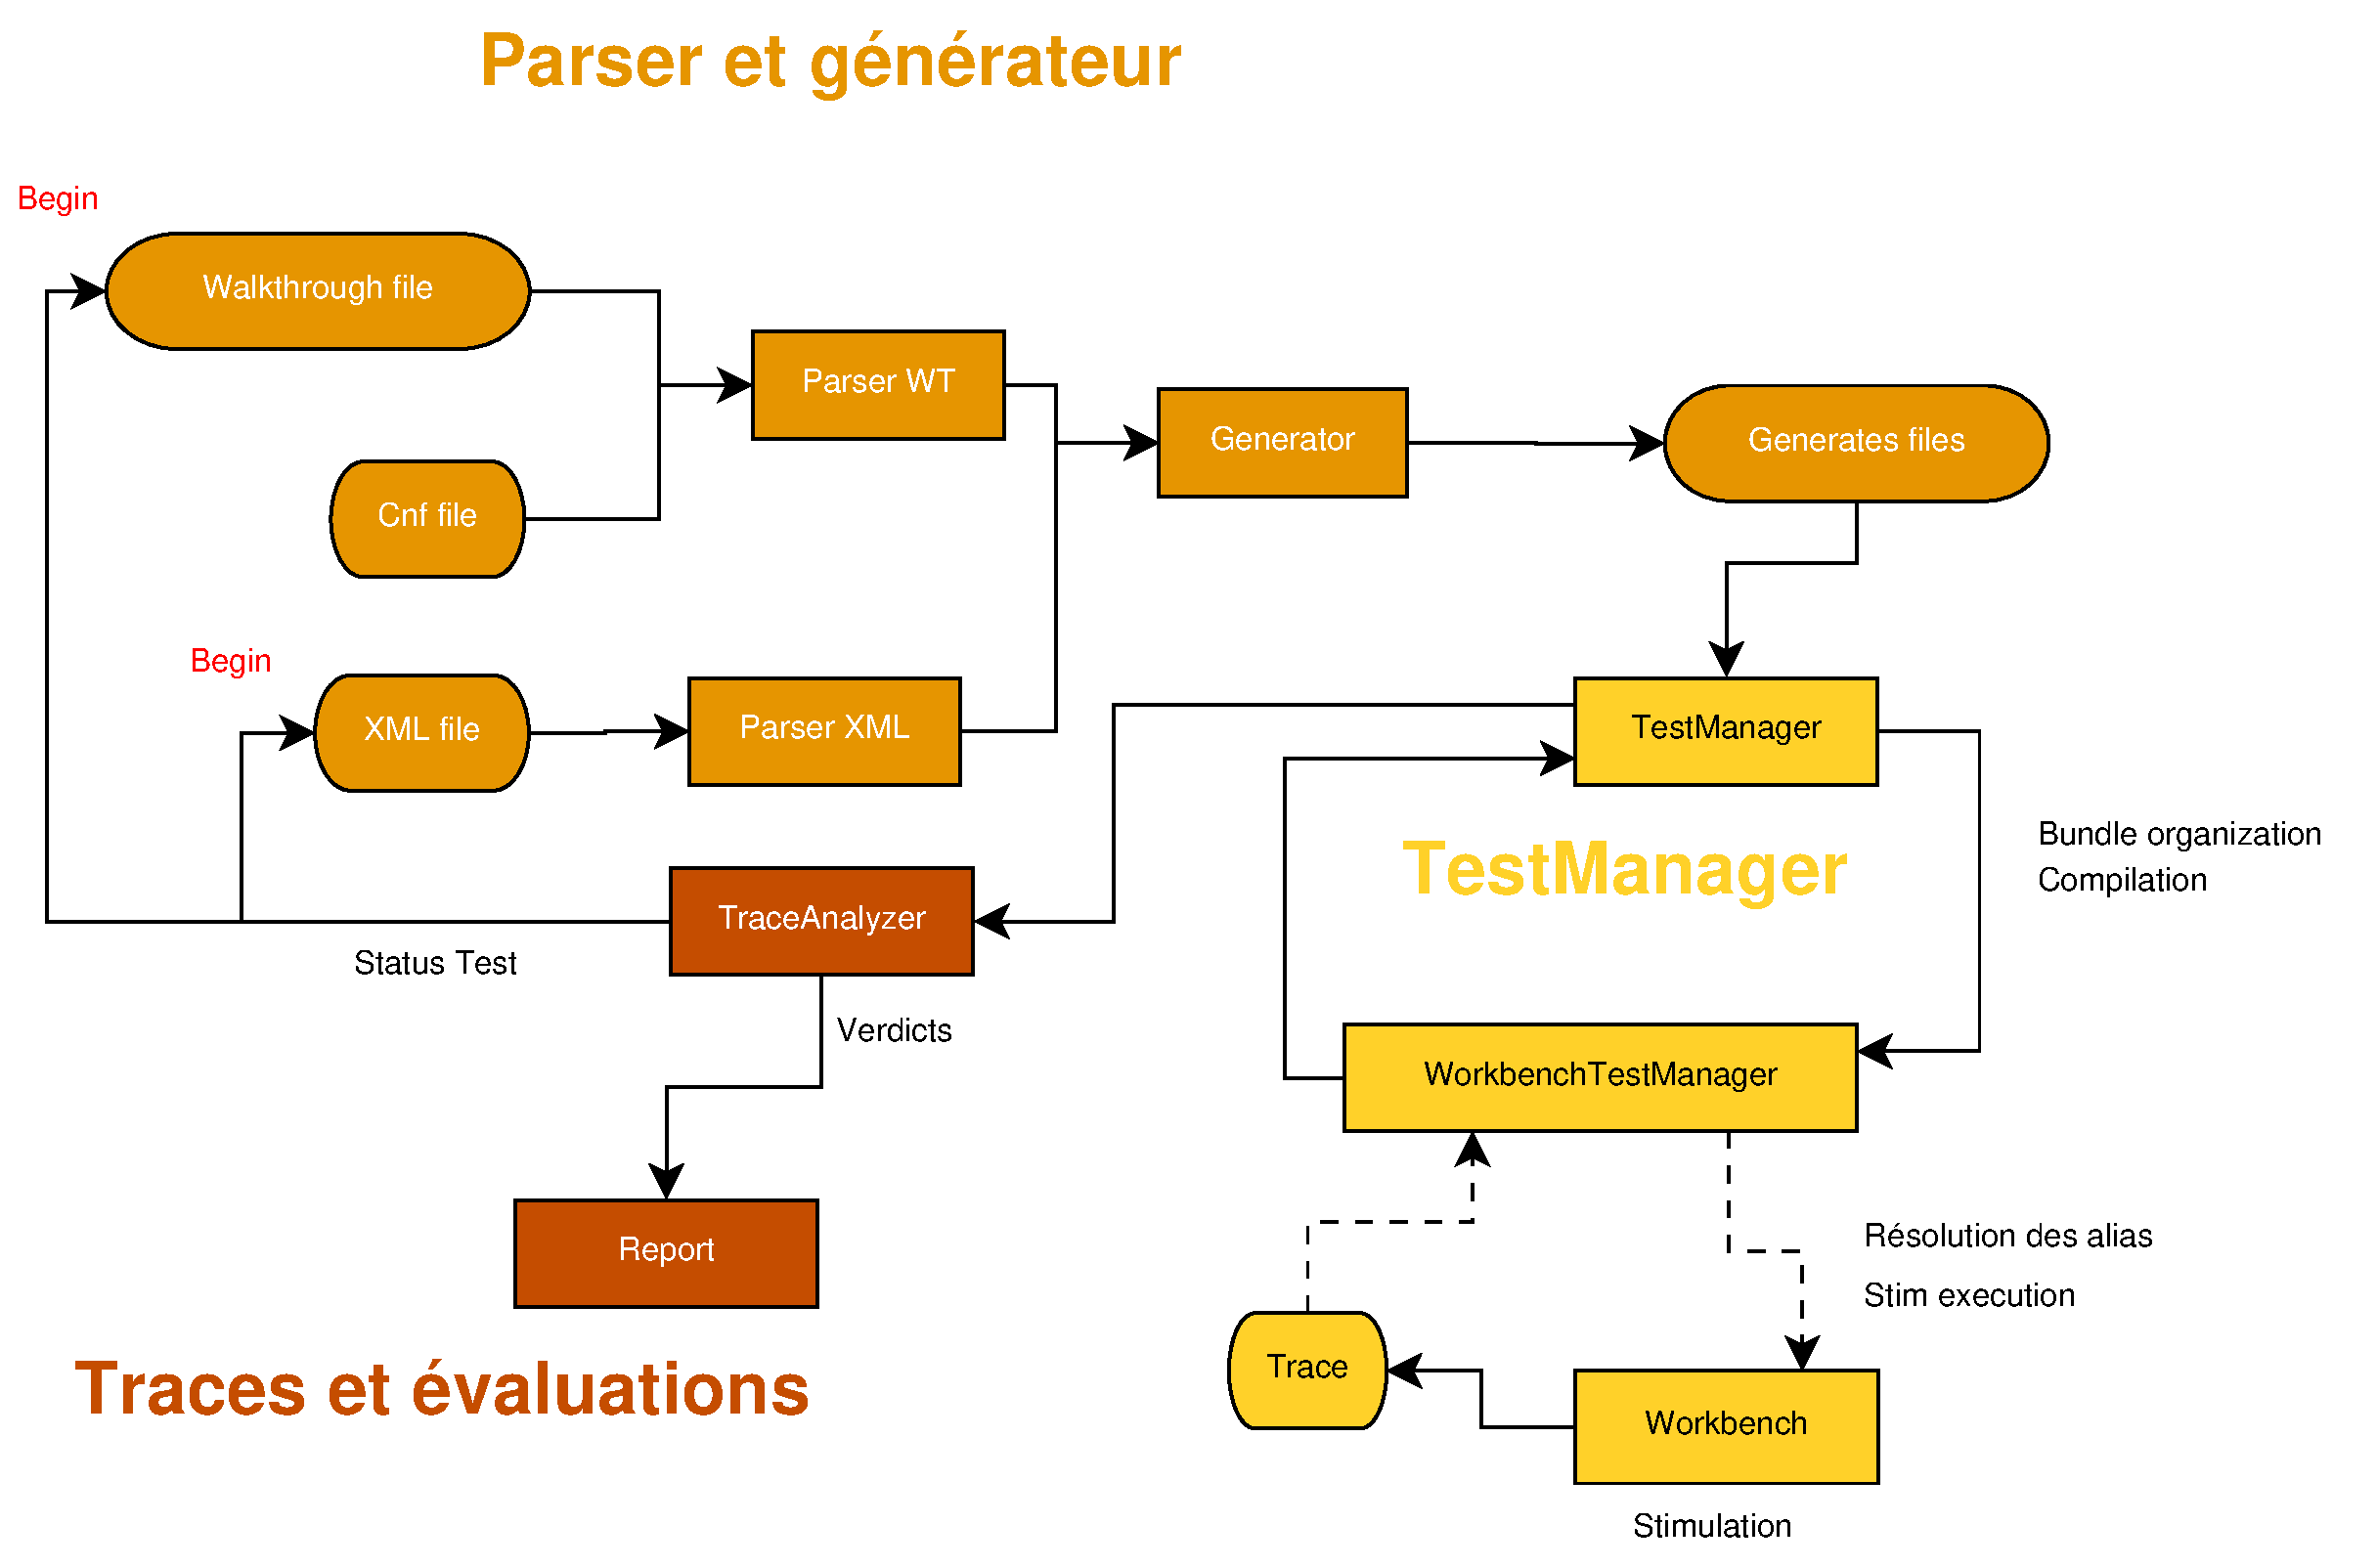
\includegraphics[width=16.5cm]{contents/images/generalDiag.eps}
			\caption{Fonctionnement général de la plateforme \textit{GreenT}}
			\label{fig:generalDig}
		\end{figure}	

	\subsubsection{Parsing et Génération}\label{generation}
	Le but premier de la plateforme est d'effectuer des tests automatiques, il est ainsi indispensable d'avoir un système d'automatisation.

	Pour cela, nous avons un parser : il analyse un certain type de fichier\footnote{Nous ne commencerons qu'avec le Walkthrough pour débuter, mais dans le futur nous pourrions avoir des fichiers XML, des bases de données, \ldots} et en retire pour chaque test, le scénario de pré condition, les différents scénarios de stimulations, leurs \textit{Expected Behavior}, les données qui devront être enregistrées ainsi que différentes information sur le test\footnote{Responsable du test, sévérité, commentaires, nom de la variable, \ldots}.

	Une fois toutes ces données acquises, il les transmet à un générateur qui est en charge d'écrire les fichiers Java de chaque test, tous sont organisés dans un dossier temporaire avec un dossier par test. Le \texttt{TestManager} peut ensuite traiter ces données.

	\subsubsection{Stimulation} \label{stim}
		Afin de tester une variable du plugin, les développeurs vont utiliser des alias présents sur un device : actuellement, un HIL ou un debugger, prochainement nous pourrions en utiliser d'autres que ces deux derniers.

		Le spécifieur va rédiger des scénarios de stimulation, ceci afin de mettre le contrôleur dans certaines conditions. Son but sera ensuite de vérifier que ces variables restent cohérentes vis-à-vis du scénario effectué. 

		Un scénario particulier doit être spécifié : une pré condition qui a pour but d'initialiser les \textit{devices} et certains alias afin d'avoir un état de stimulation qui soit cohérent et identique à chaque lancement du scénario. Ce scénario sera effectué avant le lancement de chacun des scénarios de stimulation.

	\subsubsection{Les traces et leurs évaluations}\label{expectedBehavior}
	Lorsqu'un scénario de stimulation s'exécute, un certain nombre de variables sont enregistrées : ces variables sont stockées sous la forme d'une trace au format CSV, qui pourra plus tard être représentée sous forme de courbe. 

	Une fois que la trace est complète, il est nécessaire de l'évaluer : le spécifieur a décrit le comportement attendu dans la colonne \textit{Expected Behavior} détaillant dans quel cas le test est correct, ainsi cette expression va être transformée en arbre logique afin de l'évaluer à tout instant de la trace. 

	\subsubsection{Le module TestManager}\label{testManager}
	Le \texttt{TestManager} est le chef d'orchestre de \textit{GreenT}, il a donc un certain nombre de responsabilités. 

	Il va d'abord organiser les différents tests en un concept que nous avons appelé \textit{Bundle} : afin de limiter le temps d'exécution qui atteindra plusieurs dizaines d'heures, il est intéressant de regrouper les tests possédant les mêmes scénarios de stimulations et les mêmes pré conditions. Seules leur \textit{Expected Behavior} changent, mais celles-ci pourront être évaluées sur la même Trace.

	Une fois les tests organisés en Bundle, il va les compiler et les donner à un \texttt{WorkbenchManager} : toujours pour une raison d'optimisation, il sera intéressant de pouvoir exécuter les enregistrements sur plusieurs bancs simultanément, pour cela le \texttt{TestManager} sera capable de savoir quels bancs peuvent être utilisés et pourra distribuer ses bundles en fonction. 

	Chaque \texttt{WorkbenchManager} sera en charge d'exécuter le code généré plus tôt et dialoguera en réseau avec son banc, une fois l'exécution terminée, il obtiendra une trace qui pourra être évaluée.

	Afin d'être le plus souple possible, il existe plusieurs modes d'exécution du \texttt{TestManager} : 
	\begin{description}
		\item[Check only] Essaye de parser les différents fichiers, et vérifie que ceux-ci ne comportent aucune erreur de grammaire, d'alias introuvable, d'écriture sur un alias en lecture seule etc...
		\item[Parse and generate jar tests] Parse les fichiers et génère des jars exécutables pour chacun des tests
		\item[Parse and generate bundles] Parse les fichiers et génère des jars exécutables répartis en bundle
		\item[Parse and execute] Parse les fichiers, génère les jars pour les bundles et les exécute : c'est le mode << classique >>.
		\item[Restart test execution] Redémarre une exécution qui se serait mal terminée.
	\end{description}
	\subsubsection{Production de rapport détaillé}\label{report}
	La plateforme a en charge la production d'un rapport détaillé pour chaque test. Ce rapport contiendra un certain nombre d'informations, et permettra au testeur de comprendre pourquoi le test n'est pas passé. Voici les informations que contiendra ce rapport : 

	\begin{itemize}
		\item Nom du test, de la variable à tester
		\item Nom du responsable du test
		\item Sévérité du test
		\item Pourcentage de branches de l'expectedBehavior renvoyant faux(Test << Rouge >>), n'ayant pas pu être testé(Test << Gris >>) et étant correct(Test Vert)
		\item Le testeur aura à sa disposition les expressions concernées par un résultat Rouge ou Gris.
		\item Les colonnes utiles du \texttt{Walkthrough}
	\end{itemize}

	Actuellement, les rapports se font au format Excel avec l'intégralité de notre enregistrement et pour chaque timestamp, un verdict. Un exemple de rapport est accessible en Annexe TODO. 
	
	Dans un futur proche, ces rapports pourraient être générés dans un format Web avec une possibilité de naviguer entre plusieurs tests, et d'avoir un affichage des courbes de manière graphique.

	\subsubsection{Mise à jour du Walkthrough}
	Une fois un test exécuté, un résultat est mis dans le fichier Excel, en fonction de l'analyse précédemment de la trace : un verdict rouge renverra un résultat rouge, si tout est vert le résultat vert et enfin, celui-ci pourra être gris si nous n'avons pas été capable d'evaluer de résultats.
	


	\setcounter{mtc}{8}
	\chapter{Ma collaboration au projet}\label{collab}
\putminitoc
Après avoir défini plus en détails les besoins de notre plateforme et son fonctionnement général, nous allons maintenant voir en détail de quelle manière j'ai contribué à ce projet. En parallèle de la maintenance de notre plateforme, j'ai développé deux nouvelles fonctionnalités. Ces deux fonctionnalités ayant un rapport direct avec la notion de << calibration >>, nous allons tout d'abord définir celles-ci avant de voir en détail mon développement et la maintenance que j'ai effectué.

\section{Les calibrations}
Une calibration est une constante stockée en flash, c'est-à-dire en mémoire non volatile. Ainsi le logiciel du contrôle moteur peut accéder à toutes ces calibrations en lecture uniquement.

Ces calibrations permettent de configurer un véhicule avant sa mise en production. Cette configuration peut se faire en fonction de plusieurs critères : 
\begin{itemize}
	\item Le matériel en face du calculateur, comme le nombre d'injecteurs
	\item La version du logiciel du contrôle moteur
	\item Leur modification permet de faire une mise au point, permettant d'améliorer la consommation par exemple.
\end{itemize}

Une fois le logiciel d'un calculateur mis en production, ces calibrations ne doivent pas évoluer, les modifier ne sert donc qu'à la mise au point et à la généricité du logiciel.

\section{Le << patch calib >>}\label{patch}
Pour un certain nombre de scénario de stimulation, il est nécessaire de modifier des valeurs de calibrations. Cette action demande d'ajouter une grammaire spécifique : \texttt{PATCH\_CAL(calibration, valeur)}. En interne, cela générera du code permettant de flasher la nouvelle valeur.

\subsection{Expression du besoin}\label{besoinArray}
\subsubsection{Les cas d'utilisation}

\begin{figure}[H]
\includegraphics[width=16cm]{contents/images/patch-calib.jpg}
\end{figure}

\subsubsection{Les limitations de la fonctionalité}
Afin de pouvoir patcher des calibrations, j'ai du me renseigner auprès de personnes compétentes et sachant comment cela pouvait se faire. Il s'est trouvé que nous allons devoir adapter un script déjà existant.

Cepepdant, afin de pouvoir modifier la flash, il est indispensable que notre ECU soit arrêté, ainsi il ne sera possible de ne modifier des calibrations qu'en début de scénario. L'utilisateur modifie ces éventuels calibrations puis effectue son scénario de stimulation. Cette restriction n'est pas incensée, en effet, afin de tester correctement le programme il doit être dans des conditions les plus proches du réel. Or, sur une voiture, il n'est pas possible de modifier des calibrations avec l'ECU démarré.

Si pour un test, l'utilisateur veut vérifier que tout s'exécute correctement avec différentes calibrations, il pourra utiliser plusieurs scénarios : un scénario par groupe de calibrations. 

\subsection{Fonctionnement à l'utilisation}
Comme vu section \ref{besoinArray}, le << patch calib >> ne peut être utilisé que si l'ECU est arrêté. Afin de forcer ce fonctionnement, et d'éviter une mauvaise utilisation, il a été choisi d'utiliser la grammaire du langage. En effet, une mauvaise utilisation de la fonctionnalité nous renverra une \textit{syntax error}, forçant l'utilisateur à corriger cela. 

\begin{lstlisting}[language=gtl,numbers=left,caption=Scénario de stimulation contenant des patchs de calibration]
SCENARIO NomDuScenario
  PATCH SECTION
    patch_cal(cal1, value1);
    patch_cal(cal2, value2);
  END SECTION
  // Stimulation proprement dite
  // Rampe, wait, ...
END SCENARIO
\end{lstlisting}
L'utilisateur à la possibilité d'écrire plusieurs scénarios dans un même test, avec cette même syntaxe.

\subsection{Conception de la solution}

\section{Les << tableaux calibrables >>}
Certaines variables côtés ECU sont des variables de types tableau, l’utilisateur peut actuellement y accéder via la syntaxe \texttt{var[indice]}.

Le but de mon développement, était d’améliorer ce système. Actuellement, seul un indice en dur peut être renseigné à cette variable, l’idée est de pouvoir renseignée un indice en dur, mais aussi une calibration.

\subsection{Expression du besoin}\label{besoinTab}
Cette fonctionnalité permettrai d’avoir des calibrations d’un projet à l’autre, et de pouvoir réutiliser le \textit{Walkthrough} en ne changeant que les calibrations.\\
Un autre intérêt de cette fonctionnalité, est de pouvoir recopier les spécifications, celles-ci étant renseignée via des calibrations.

Avec cette fonctionnalité, l'utilisateur pourra donc avoir des fichiers \textit{Walkthrough} génériques et réutilisable entre chaque versions d'un même projet. Cela limiterai également le risque d'erreur dûe à une mauvaise recopie de la spécification. En effet, avant cette fonctionnalité, l'utilisateur devait regarder la spécification, aller voir le contenu de la calibration, et la mettre en dur dans le test. Cela peut provoquer des erreurs, d'une part lors de la recopie de la valeur, mais également si la valeur change à la version suivante et que l'utilisateur ne pense pas à faire suivre son document. 

\subsubsection{Les cas d'utilisation}
\subsubsection{Les limitations de la fonctionalité}


\section{La maintenance}
Comme expliqué plus haut, j'ai développé deux fonctionnalités durant ce stage. Cependant, en parallèle de ce développement j'ai également corrigés différents bogues, ou améliorer différentes partie de la plateforme.

Ayant conçu cette plateforme lors de mon stage de fin de Licence, je connais l'intégralité de la plateforme. C'est ainsi que j'ai pu détecter et corriger un certains nombres de problèmes. Ces bogues ou ces améliorations ont été identifiées de trois façons différentes : 
\begin{itemize}
	\item Durant mon développement, il m'est arrivé de trouver du code incohérent ou bouchonné
	\item Lors d'exécutions de la plateforme sur différentes versions du projet client
	\item En regardant les différents tickets ouverts et devant être résolus
\end{itemize}

\subsection{Corrections}
J'ai corrigé quelques problèmes trouvés sur la plateforme, principalement venant du client \textit{GreenT}. Ceci étant dû à notre choix d'architecture : des serveurs les plus légers et un client effectuant le maximum d'actions.
	\subsubsection{Stockage des erreurs d'exécutions}
	\begin{description}
		\item[Le problème] En cas d'erreur durant une exécution, si un serveur ne répond plus, si une variable est non trouvée, ... Une exception est levée. À ce moment là, \textit{GreenT} doit attraper l'exception et la stocker en base de données pour pouvoir afficher ensuite le message à tous les tests du bundle, la génération des rapports ne pouvant pas se faire.
		\item[La solution] Le stockage du message d'erreur n'était pas fait, ainsi que la requête SQL permettant d'obtenir les messages d'erreurs. Ces deux actions ont été corrigés, en lieu et place du rapport de test nous avons maintenant un message d'erreur clair.
		\end{description}
		
	\subsubsection{Modification des variables Debugger}
		\begin{description}
			\item[Le problème] Lors d'un stimulus, il est possible de modifier une variable Debugger. Lors de la modification d'une variable, le Trace32 renvoyait toujours une exception, sans appliquer la modification.
			\item[La solution] Après lecture de la documentation de Trace32, il s'est avéré que le problème venait simplement du serveur qui appliquait une commande syntaxiquement incorrecte. La modification de la commande a corrigé le problème.
	\end{description}
	
	\subsubsection{Ordre d'exécutions des scénarios}
		\begin{description}
			\item[Le problème] Un Test peut contenir plusieurs scénarios, ceux-ci nous servent principalement pour le << patch-calib >> comme expliqué section \ref{patch}. Or, si nous utilisions plusieurs scénarios, ceux-ci étaient exécutés dans un ordre aléatoire : si l'utilisateur voulait effectuer des actions dans un ordre donnée, ce n'était pas possible.
			\item[La solution] Le problème avait deux parties : d'une part, l'exécution des scénarios dans un ordre donné, d'autre part, spécifier un ordre à chacun de nos scénarios. En effet, tout d'abord, j'ai nommé les scénarios de sortes qu'ils soient classé par ordre alphabétique. Ensuite, il a fallu spécifier à la plateforme d'exécuter les différents scénarios dans un ordre alphabétique, pour cela il a suffit d'utiliser une collection Java effectuant cette action, la \texttt{TreeMap}.
	\end{description}
	
	\subsubsection{Reset ECU à l'exécution}
	\begin{description}
		\item[Le problème] Lors de l'exécution de notre plateforme sur la dernière version du projet client, nous avions systématiquement un \textit{reset} ECU. C'est-à-dire que notre ECU s'arrêtait et ne redémarrait pas pour une raison inconnue.
		\item[La solution] Le problème ne venait pas directement de la plateforme, mais d'une mauvais configuration de notre part. En effet, nous ne spécifions pas les bons fichiers du logiciel, celui-ci étant mal flashé, l'ECU refusait de démarrer.
	\end{description}
	
	\subsubsection{Absence d'injection}
	\begin{description}
		\item[Le problème] Lorsque j'essayais de simuler un démarrage du moteur sur la dernière version du logiciel, aucune injection ne se faisait : après le starter, le moteur retournait à zéro tour.
		\item[La solution] Après s'être renseigné auprès de personnes compétentes, il s'est avéré que cela venait d'un nouveau fichier à flasher dont nous n'avions pas connaissance. Un fichier contenant des calibrations permettant le démarrage du moteur sur table. Ce fichier n'ayant pas été pris en compte durant la conception, j'ai ajouté un nouveau paramètre au fichier de configuration permettant de renseigner des fichiers à flasher additionnels.
	\end{description}
	
\subsection{Améliorations}
	\subsubsection{Exécution différée} %
	\begin{description}
		\item[Le besoin] Lors de mon développement, j'ai eu souvent des problèmes pour réservés des tables de tests. Celles-ci étant régulièrement prise par les équipes projets. 
		\item[La solution] Afin de ne pas bloquer de tables, et de ne pas bloquer notre travail en raison de l'absence de celles-ci, une solution nous est venue : la possibilité de lancer l'outil durant la nuit. En effet, actuellement une exécution dure environ 45 minutes, après laquelle nous pouvons analyser les rapports et voir les problèmes qui nous sont retournés. Ainsi, j'ai ajouté un nouveau paramètre à l'application permettant de spécifier l'heure à laquelle la génération des \texttt{.jar}, la compilation, l'exécution et la génération des rapports va se faire. On peut maintenant lancer une exécution le soir et observer les résultats le lendemain matin.
	\end{description}
	
	\subsubsection{Passage à Java 8}
		\begin{description}
			\item[Le besoin] La plateforme fonctionnait sous Java 6. Ainsi, nous allions mettre en production une plateforme déjà obsolète à sa sortie. De plus, les deux versions suivantes de Java propose un certain nombre de fonctionnalités aidant au développement, comme des simplifications d'écriture en Java 7 (\textit{Multi-Catch}, Inférence de type, \texttt{switch} sur les strings, ...) ou les lambdas-calculs en Java 8. Enfin, dans un future proche nous aurons besoin d'une interface pour \textit{GreenT}, \texttt{JavaFx} serait une bonne solutions, mais celle-ci nécessite Java 8.
			\item[La solution] Avant de passer à Java 8, il a d'abord fallut vérifier qu'aucune incompatibilité avec les bibliothèques que nous utilisons n'allait apparaître. Ensuite, il était nécessaire de télécharger un compilateur ainsi qu'une JVM, configurer les différents environnements et vérifier qu'une exécution se passait de la même manière que précédemment. Après ce succès, le passage à Java 8 a été concrétisé et permet à notre plateforme de rester moderne ! 
		\end{description}
		
	\subsubsection{<< \textit{Clean-Code} >>}
		\begin{description}
			\item[Le besoin] \textit{GreenT} ayant deux ans, et ayant connue quatre développeurs différents, il est parfois nécessaire d'améliorer le code existant ou de le rendre plus lisible. 
			\item[La solution] Lorsqu'en développant mes fonctionnalités ou en corrigeant des bugs je tombais sur du code incompréhensible ou du << code mort >>, je modifiais celui-ci afin de corriger ces défauts. Ceci permet ainsi de garder un code toujours propre et facile à lire.
		\end{description}
		
	\subsubsection{Affichage des \textit{logs}}
		\begin{description}
			\item[Le besoin] La plateforme effectue beaucoup d'actions, allant du parsing jusqu'à la génération des rapports comme montré chapitre \ref{chapGreent}. Toutes ces actions doivent être tracés, aussi bien en temps réel, en regardant l'exécution, que plus tard en observant un fichier.
			\item[La solution] Les logs fonctionnait déjà, en utilisant \texttt{log4j}, cependant celui-ci affichait beaucoup trop d'informations en temps réel, et n'affichait pas les informations les plus utiles. Ainsi, j'ai passé en revue la plateforme pour afficher les bonnes actions (Initialisation des bancs, stimulis effectués, affichage des exceptions, \ldots). Toutes les erreurs sont redirigé vers la sortie des erreurs (\texttt{stderr}), et seules les informations les plus importantes sont sur la sortie console (\texttt{stdout}). Tous les autres logs, qui peuvent être utile à la compréhension d'un problème et nous aider ne sont accessible que dans nos fichiers de logs. J'ai par ailleurs ajouté un « buffer tournant » permettant aux fichiers de logs de ne jamais dépasser une certaines taille (5Mio), afin de ne pas consommer trop d'espace.
		\end{description}
		


	\setcounter{mtc}{9}
	\chapter{Bilans}
\putminitoc

Après ce stage de quatre mois, il est temps de dresser un bilan, du point de vue de Continental, ce que mon travail leur a apporté, mais également en quoi ce stage a été bénéfique pour ma future carrière professionnelle.

\section{Bilan pour Continental}
Mon travail dans l'équipe de développement aura été intéressant pour l'entreprise, en partie grâce à ma connaissance de la plateforme suite à mon stage de licence. En effet, avoir contribué au projet l'année précédente sur la conception de celui-ci m'a permis de rapidement commencer le travail et de corriger des bugs répartis dans différents modules. De plus, revenir huit mois plus tard sur ce projet m'a permis d'appréhender le logiciel de manière plus globale et j'ai ainsi pu soulever des problèmes que nous n'avions pas vu lors de la conception.

Grâce à mes connaissances de l'architecture j'ai aidé Benjamin \bsc{Guerin} -- le troisième membre de l'équipe arrivant sur le projet -- j'ai ainsi pu lui donner des explications et des conseils, pendant que lui apportait un regard neuf à l'existant.

Comme présenté chapitre \ref{collab}, mon travail aura été directement utile à l'équipe de développement, et au groupe TAS. En effet, j'ai développé deux nouvelles fonctionnalités attendues par le client mais j'ai également corrigé des bugs. Ces corrections de bugs ainsi que les nouvelles fonctionnalités nous permettent maintenant d'exécuter les stimulations ainsi que l'analyse complète sur la dernière version du projet Ford : il est maintenant possible d'avoir les résultats de XX tests en une heure.

Le projet n'est pas terminé, et je n'ai pas pu effectuer toutes les fonctionnalités auxquels nous avions pensés tel que l'utilisation de GreenT avec d'autres fichiers d'entrées que le Walkthrough. Ceci est principalement due à de mauvaises estimations, notamment en raison de la maintenance demandant plus de temps que prévu. Cependant, je vais continuer ce projet dès septembre en contrat de professionnalisation pendant un an et pourrais ainsi finaliser la plateforme.

\section{Bilan personnel}
% 	Cette expérience en entreprise m'a beaucoup apporté, tout d'abord d'un point de vue technique, j'ai acquis de l'expérience en conception logicielle, grâce
% 	à toutes nos réunions où nous réfléchissions à la meilleure approche possible. De plus lors de problèmes, les propositions des autres m'ont permis d'avoir
% 	une autre vision du problème et une autre manière de le résoudre !

% 	Mais j'ai aussi acquis des connaissances humaines avec notamment le travail en équipe, communiquer sur nos avancements, et être capable de synthétiser ses
% 	propositions ou de réussir à poser un problème rapidement tout en se faisant comprendre.

% 	Ce stage m'a permis de découvrir le monde d'une grande multinationale. Jusqu'à maintenant je ne connaissais que les PME et je n'étais pas sûr de pouvoir
% 	travailler dans une grande entreprise.

% 	Un bilan très positif, qui m'a réconforté dans mon projet professionnel : le développement logiciel et la conception sont vraiment les domaines de
% 	l'informatique qui m'intéressent le plus, je souhaite poursuivre vers un master Développement Logiciel.


	\appendix
	\mystarpart{Annexes}{\hfill\begin{minipage}{0.5\textwidth}Ci-après vous trouverez un certain nombre d'annexes qui pourront vous permettre de mieux comprendre l’étendue de mon travail et de la plateforme qui est en cours de développement.\newline~\newline			
			Vous y trouverez ainsi un glossaire, des références, des exemples de rapport, de fichiers générés ainsi qu'une explication plus approfondie des équipements utilisés.\end{minipage}}

	\chapter{Acronymes et Glossaire}\label{glo}
\begin{description}
\item[API] Application Programming Interface, ensemble normalisé de classes, de méthodes ou de fonctions qui sert de façade par laquelle un
	logiciel offre des services à d'autres logiciels.
	\item[Analyseur logique] L'analyseur logique est un outil de mesure permettant de connaître au fil du temps l'évolution binaire des signaux (0 et 1) sur plusieurs voies logiques : bus de données, entrées-sorties d'un microcontrôleur ou d'un microprocesseur.
\item[Antlr] \textit{Another Tool for Language Recognition}, outil permettant de faciliter l'interprétation d'une chaîne de caractère, celui-ci prend en entrée une
	grammaire, et génère un arbre syntaxique dans plusieurs langages.
\item[Calibration] Valeur stockée en flash pouvant contenir une information permettant de simplifier la configuration véhicule. Une
	calibration pourrait être le nombre d'injecteurs.
\item[CAN] \textit{Controller Area Network}, un bus système série très répandu dans beaucoup d'industries, notamment l'automobile. Ce bus permet de racorder à un même bus un grand nombre de calculateurs qui communiqueront à tour de rôle.
\item[ControlDesk] Outil permettant de piloter le HIL, l'interface permet ainsi de modifier des valeurs de l'environnement véhicule, ou de
	pouvoir les lire graphiquement.
\item[Device] Les différents équipements dont pourrait avoir besoin l'utilisateur : Hil, Debugger, \ldots 
\item[ECU] Electronic Control Unit, calculateur du contrôle moteur
\item[Excel] Logiciel tableur appartenant à la suite de Microsoft Office\textregistered. Il est possible de modifier une feuille de calcul depuis un logiciel ou un script, notamment en Java. 
\item[Flash] La mémoire flash est une mémoire de masse non volatile et réinscriptible. Ainsi les données sont conservées même si l'alimentation est coupée.
\item[Flasher] Action d'écrire sur la flash, dans notre cas il s'agit d'écrire ou de mettre à jour le logiciel présent sur la mémoire flash de l'ECU.
\item[Grammaire] Formalisme permettant de définir une syntaxe clair et non ambigüe.
\item[HiL] \textit{Hardware in the loop}, permet de simuler un environnement véhicule autour du calculateur du contrôleur moteur : celui-ci réagira comme s'il était embarqué dans une voiture.
\item[JAR] Java ARchive est un fichier ZIP utilisé pour distribuer un ensemble de classes Java.
\item[Java] Langage de programmation orienté Objet soutenu par Oracle. Les exécutables Java fonctionnent sur une machine virtuelle Java et permettent d'avoir un
	code qui soit portable peut importe l'hôte.
\item[JSON] JavaScript Object Notation est un format de données textuelles, générique, dérivé de la notation du langage JavaScript, il permet de représenter de
	l'information structurée.
\item[JVM] \textit{Java Virtual Machine}
\item[Lauterbach] Société allemande spécialisée dans les outils de debuggage de systèmes embarqués. Nous utilisons leur debugger, ainsi que leur analyseur logique.
\item[Logiciel de versionnement] Logiciel, tel que \textit{Git}, permettant de maintenir facilement toutes les versions d'un logiciel, mais aussi facilitant le
	travail collaboratif.
\item[Parsing] Processus d'analyser de chaîne de caractère, en supposant que la chaîne respecte un certain formalisme. 
\item[Python] Langage intérprété de programmation multi-plateforme et multi-paradigme. Il est doté d'un typage dynamique fort, d'une gestion automatique de la mémoire et d'un système de gestion d'exceptions. 
\item[Release] Version d'un logiciel qui correspond à un état donné de l'évolution d'un produit logiciel utilisant le versionnage. Ainsi, chez Continental, un projet comporte une multitude de versions différentes.
\item[Apache Thrift] Langage de définition d'interface conçu pour la création et la définition de services pour de nombreux langages. Il est ainsi possible de
	faire communiquer deux problèmes dans deux langages différents : Python et Java dans notre cas.
\item[Trace32] Debugger, permet de debugger un programme embarqué, ceci en permettant de lire la mémoire, mettant des points d'arrêts, \ldots
\item[UML] Unified Modeling Language est un langage de modélisation graphique. Il est utilisé en développement logiciel et en conception orienté Objet afin de
	représenter facilement un problème et sa solution.
\item[XML] Extensible Markup Language est un langage de balisage générique permettant de stocker des données textuelles sous forme d'information structurée.
\end{description}


	\printindex
	\chapter{Références}\label{references}	
Voici les références que j'ai utilisées durant ce stage : particulièrement de la documentation, quelques livres dans lesquels j'ai lu les chapitres qui m'intéressaient pour résoudre un certain problème, certains cours enseignés durant mon cursus, et enfin des sites web et forums me permettant de résoudre des problèmes spécifiques.

\section{Documentations}
\subsection{En ligne}
\begin{description}
	\item[Documentation Thrift] \url{https://thrift.apache.org/docs/}
	\item[Documentation Antlr] \url{http://www.antlr.org/api/}
	\item[Documentation Freemarker] \url{http://freemarker.org/docs/}
	\item[Documentation Git] \url{http://git-scm.com/documentation}	
	\item[Documentation Java] \url{http://docs.oracle.com/javase/6/docs/api/}
	\item[Documentation Python] \url{https://docs.python.org/2.6/}
\end{description}

\subsection{Chez Continental}
\begin{description}
	\item[Documentation Lauterbach] Documentations sur le fonctionnement du debugger lauterbach, du langage de scripts ainsi que de l'analyseur logique.
	\item[Documentation ASAP2] Documentation sur la norme ASAP2, notamment utilisée pour la rédaction de fichier A2l.
	\item[Documentation Infineon] Documentation permettant de comprendre globalement le fonctionnement du calculateur, et permettant de comprendre des problèmes posés par le debugger Lauterbach.
\end{description}

\section{Livres}
	\begin{description}
	\item[UML2 par la pratique -- \'Etude de cas et exercices corrigés] sixième édition, 2008. Rédigé par Pascal \bsc{Roques}
	\item[Design Patterns : Elements of Reusable Object-Oriented Software] Second edition, 1999. Rédigé par le Gang of four : Erich \bsc{Gamma}, Richar \bsc{Helm}, Ralph \bsc{Johnson} et John \bsc{Vlissides}.	
		\item[The definitive Antlr4 reference] 2013, Rédigé par Terence \bsc{Parr}
	\item[The \LaTeX{} Companion] 2nd édition, 2004. Rédigé par Franck \bsc{Mittelbach}, Michel \bsc{Goossens}, Johannes \bsc{Braams}, David \bsc{carlisle} et Chris \bsc{Rowley} 
\end{description}
\section{Cours magistraux}
\begin{description}
	\item[Design patterns] 2015, M1 Informatique Développement Logiciel, Jean-Paul \bsc{Arcangeli}
	% TODO Cours M1 de cher-cher
	% TODO Cours de M2 ? 
%	\item[
	\item[Modélisation Conception Programmation Orienté Objet] 2014, M1 Informatique, Ilena \bsc{Ober}
	\item[Traduction de langages] 2015, M1 Informatique, Christine \bsc{Maurel}
	\item[Langages et automates] 2013, L3 Informatique, Christine \bsc{Maurel} et Jean-Paul 
		\bsc{Arcangeli}
	\item[Construction et réutilisation de composants logiciels] 2014, L3 Informatique parcours ISI, Christelle \bsc{Chaudet}
	\item[Conception UML] 2012, DUT Informatique, Thierry \bsc{Millan}
%	\item[Qualité logicielle] 2012, DUT Informatique, Thierry \bsc{Millan}
\end{description}
\section{Sites Web et forums}
	\begin{description}
		\item[StackOverflow] \url{http://stackoverflow.com}
		\item[Developpez] \url{http://www.developpez.com/}
		\item[Wikipédia] \url{http://en.wikipedia.org/wiki/}
	\end{description}


	\chapter{Exemple de rapport généré par GreenT}\label{apendixReport}
\begin{figure}[H]
\centering
\includegraphics[width=13cm]{contents/images/report.png}
\caption{Exemple d'un extrait de rapport généré par \textit{GreenT}}
\end{figure}
Ce rapport est un rapport vérifiant que la variable \texttt{EnvT\_tSens=temp\_air\_mes[2]}, moyennant une tolérance. 

\begin{itemize}
\item Dans la colonne A, nous avons le timestamp, le temps durant lequel la valeur a été enregistrée
\item Dans les colonnes B et C, nous avons la valeur de nos variables, en physique, c'est-à-dire converties par \textit{GreenT}
\item Dans les colonnes D et E, c'est la valeur hexadécimal, c'est-à-dire la valeur enregistrée. Cette valeur est reportée dans le rapport uniquement au moment ou elle à changé. ça peut permettre à l'utilisateur de connaître les instants ou une variable est modifiée.
\item Et enfin, dans la colonne F, le résultat de l'évaluation pour chaque instant de la trace; En l'occurence, il est toujours \textit{GREEN}.
\end{itemize}
	\chapter{Release note}\label{releasenote}

\begin{figure}[H]
\centering
\includegraphics[width=13cm]{annexes/GreenT_v1-1-0_DeliveryNote.pdf} 
\caption{Release note de la versions 1.1.0}
\end{figure}
		\chapter{Exemples de fichiers générés}\label{annexeGeneration}
	\section{Exemple de StimScenario}
	\lstinputlisting[language=Java,caption=Exemple de fichier de stimulation]{contents/gttest.java}
	\section{Exemple de \texttt{GreenTTest}}
	\lstinputlisting[language=Java,caption=Exemple de fichier de GreenTTest]{contents/stim.java}


	\listoffigures
	\lstlistoflistings

	
\end{document}
